\documentclass[10pt, french, a4paper]{report}

\usepackage[authoryear]{natbib}

\usepackage[textwidth=14cm]{geometry}
\usepackage{babel}
\usepackage{xcolor,graphicx}
\usepackage{hyperref}	
\usepackage{enumitem}
\usepackage{tabularx}
\usepackage{amsmath}


\renewcommand{\thechapter}{\Roman{chapter}}
\renewcommand{\contentsname}{Table des Matières}
\makeatletter
\renewcommand{\@chapapp}{Chapitre}
\makeatother

\setcounter{secnumdepth}{3}

\title{L'Ethique des Intelligences Artificielles :\newline Supervisation et confiance}
\author{Nathan Lauga}
\date{\today}

\begin{document}

% ======= PAGE TITRE ======== %

\begin{titlepage}
  \begin{center}

    
\includegraphics[height=1.3cm]{images/CEAPC_logo.png}
    \hspace{\fill}
    
\includegraphics[height=1.5cm]{images/ynov_informatique_logo.png}

    \vspace{2.5cm}
    {\scshape\LARGE Mémoire de Mastère\par}
    \vspace{1cm}
    {\scshape\Large Ynov Informatique Bordeaux\par}
    \vspace{0.5cm}
    {\scshape\large Mastère Data Science\par}
    \vspace{1cm}
    
    % Title
    \rule{\linewidth}{0.3mm} \\[0.4cm]
    { \huge \bfseries L'\uppercase{é}thique des Intelligences Artificielles \newline Supervisation et Confiance \\[0.4cm] }
    \rule{\linewidth}{0.3mm} \\[1cm]
  
    \vspace{1.5cm}

    \noindent
    \begin{minipage}{0.4\textwidth}
      \begin{flushleft} \large
        \textbf{Réalisé par :}\\
        M.~Nathan \textsc{Lauga}\\
      \end{flushleft}
    \end{minipage}%
    \begin{minipage}{0.5\textwidth}
      \begin{flushright} \large
        \textbf{Sous la direction de :} \\
        M.~Pascal \textsc{Fournier} [CEAPC]\\
        M.~Patrick \textsc{Piquart} [YNOV]\\
      \end{flushright}
    \end{minipage}\\[1cm]

    \vspace{2.5cm}

    {\scshape\Large 16 Août 2020\par}
    
  \end{center}
\end{titlepage}

\newpage
\setcounter{tocdepth}{3}
\tableofcontents

\newpage
\begin{abstract}

    Ceci est l'avant-propos.

\end{abstract}

% ====== INTRODUCTION ====== %

\newpage
\chapter*{Introduction}
\addcontentsline{toc}{chapter}{\protect\numberline{}Introduction}

\paragraph{Problématique} 
Dans un contexte où les intelligences artificielles sont omniprésentes et que les données deviennent le nouveau pétrole, est-il possible de rendre une Intelligence Artificielle socialement responsable en supervisant son éthique ? ?


% ======= ETAT DE L'ART ====== %
\chapter{\uppercase{é}tat de l'art}
\label{chap:etat_art}

\section{Les données et l'Intelligence Artificielle}
\label{sec:ia}

\begin{quotation}
  `` Si une machine peut penser, elle pourrait penser plus intelligemment que nous, et alors où devrions-nous être ? Si nous pouvions maintenir les machines dans une position servile, par exemple en coupant le courant à des moments stratégiques, nous devrions, en tant qu'espèce, nous sentir humbles. ''
\end{quotation}
\rightline{{\rm --- \citep{turing_browse_1951}}}

\paragraph{}
Le 15 mai 1951, Alan Turing, considéré comme le père de l'informatique, été interviewé par la BBC et annoncé déjà l'avènement probable des machines intelligentes, où plus particulièrement les machines pensentes. Bien qu'à cette époque nous étions loin des ordinateurs de nos jours, la force des propos de Turing montre que, dès la moitié du 20\textsuperscript{ème} siècle, le concept d'intelligence artificielle existait.

\paragraph{}
\underline{Intelligence artificielle :} En informatique, la recherche sur l'intelligence artificielle ou IA, est définie comme l'étude des ``agnets intelligents'', soit n'importe quel appareil qui perçoit son environnement et prend des déisions qui maximisent ses chances d'atteindre son objectif \citep{poole_computational_1997}. e.g. Dans les jeux d’échecs, un agent intelligent pourra, en connaissant les règles du jeu, effectuer des coups et son objectif, sera de battre son adversaire.

\subsection{La préface : Test de Turing, Systèmes Experts et les Hivers}

\paragraph{}\underline{Algorithme :} Un algorithme correspond à une suite d'instruction pouvant exécuter une tâche précise, en informatique ce qui est appelé programme est un ensemble d'algorithme et il est de même pour les intelligences artificielles.

\paragraph{}
Intelligence Artificielle, terme qui aujourd’hui, est très évocateur, a été utilisé pour la première fois en 1956 par John McCarthy, lors de la conférence de Darthmouth, conférence qui est considérée comme l’acte de naissance de l’intelligence artificielle en tant que domaine de recherche autonome \citep{solomonoff_time_1985}. Avant cela, l'utilisation de cette notion existait déjà et l'un des premiers articles discutant de cela remonte à 1945 avant même la première explosion atomique \citep{bush_as_1945}. Dans cet article, nous pouvons y voir les concepts d'ordinateurs, d'Internet ou encore de reconnaissance vocale.

\paragraph{}
En 1948, Robert Wiener, professeur au Massachusetts Institue of Technology (MIT) théorise la Cybernétique dans son livre ``Cybernétique ou la communication contrôlée dans le domaine de l'animal et de la machine''. Il décrit une théorie entière de la commande et de la communication, aussi bien chez l'animal que dans la machine \citep{wiener_cybernetics;_1961}. La but essentiel de la cybernétique est de comprendre et de définir des processus ou fonctions avec pour objectif de réagir par rapport à une certaine action en entrée. Il s'agit là de la préface au domaine de recherche de l'Intelligence Artificielle qui émergera à la conférence de Darthmouth évoquée dans le paragraphe précédent.

\paragraph{}
Lors de l'année 1950, la théorie du domaine étant à ses débuts, un nouveau papier permettra une grande avancée, celui d'Alan Turing \citep{turing_i.computing_1950}. Intitulé ``COMPUTING MACHINERY AND INTELLIGENCE''\footnote{Traduction : Les Machines Informatiques et l'Intelligence.}, il soumettra une question inédites : ``Les machines peuvent-elles penser ?''. Cette interrogation est très contradictoire, surtout en 1950, puisque le terme \textit{machine} et \textit{penser}, ne peuvent être définis d’une façon qui puisse satisfaire tout le monde. Afin de résoudre le conflit de cette contradiction, Turing a proposé une solution, élégante, étant le fameux ``Test de Turing''. 

\paragraph{}
\underline{Test de Turing :} Si une machine peut tenir une discussion avec un humain (au travers d’une messagerie par exemple), sans que la femme ou l’homme ne puisse distinguer qu’il s’agisse d’un humain ou d’une machine alors la définition du test dira que cette machine est "pensante". Il s’agit d’une proposition très importante dans la philosophie de l’intelligence artificielle \citep{pinar_saygin_turing_2000}. 

\paragraph{}
Les années suivants ces papiers, des déclarations comme ``d’ici dix ans un ordinateur sera le champion du monde des échecs'' \citep{simon_heuristic_1958} ou encore ``des machines seront capables, d’ici vingt ans, de faire tout travail que l’homme peut faire'' \citep{simon_shape_1965} crééront un engouement populaire dans le domaine de la recherche de l'Intelligence Artificielle. Ne s'agissant pas des seules déclarations à ce sujet, et celles-ci mènent à une attente très élevée concernant les possibilités des algorithmes intelligents, mais comme souvent lorsque les attentes sont élevées une phase de déception s’ensuit.

\paragraph{}
Dans les années 1970, apparu le premier hiver de l’histoire de l’intelligence artificielle. Comme une bulle qui aurait éclaté, la recherche a ralenti d’un coup, ainsi que le budget consacré au domaine. Les causes en sont multiples. Il est possible de retrouver entre autres, la limite de la puissance de calcul des ordinateurs ou encore le manque de base de connaissances du monde par les ordinateurs (manque de données). En effet, les travaux, qui portaient sur le langage naturel, ne pouvaient pas être extrêmement poussés puisque le stockage de la mémoire la limitait à vingt mots \citep{crevier_ai:_1992}. Pour beaucoup ce secteur a été enterré, mais arrivèrent les systèmes experts, programmes qui allient algorithme et connaissance métier. Ce concept qui comme le Soleil au printemps fit fondre la neige du premier hiver.

\paragraph{}
\underline{Système Expert :} c'est un programme capable de reproduire des patterns afin d'obtenir une sortie. Concrètement, c'est un logiciel qui avec une base de connaissances et une base de règle peut obtenir une réponse \citep{jackson_introduction_1998}. E.g. Un système expert peut avoir comme connaissance les polygones et leur nombre de côtés puis pour règle l'association comme trois côtés égal un triangle.

\paragraph{}
L’histoire se répéta malheureusement dans les années 90 : trop d’attente pour une réalité en dessous de l’imaginaire. La conséquence fut une nouvelle période froide dans ce domaine et un désenchantement populaire.

\begin{center}
  \begin{figure}[hbt!]
      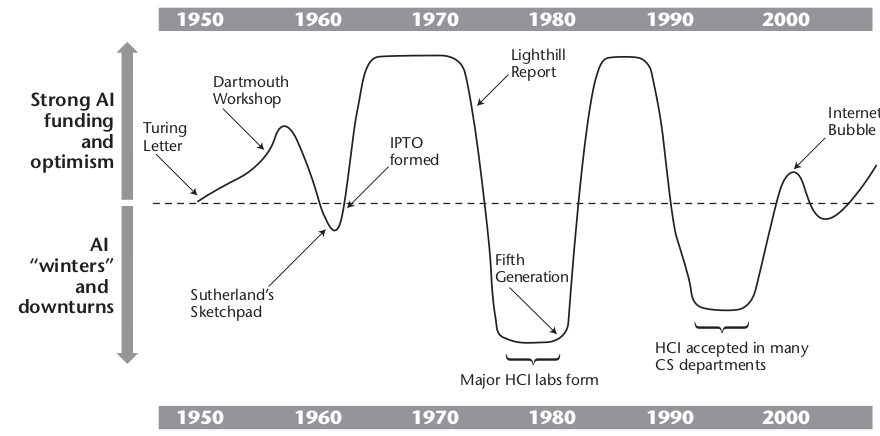
\includegraphics[width=\textwidth]{images/grudin_2009_changing_seasons_ai.png}
      \caption{Les saisons changeantes de l'IA \citep{grudin_ai_2009}}
  \end{figure}
\end{center}

\paragraph{}
Ci-dessus un résumé des débuts de l’histoire de l’intelligence artificielle avec en abscisse les années et en ordonnées l’attente autour de ce secteur. Sur le graphique, certains évènements majeurs de l’histoire du domaine en question. Aujourd'hui, grâce à plusieurs éléments l'IA retrouve une place dominante, entre autres la quantité de données à disposition a permi de faire exploser ce domaine de recherche. 

\subsection{Le changement des échelles de grandeurs : les données et Big Data}

\begin{quotation}
  ``Les données sont le nouveau pétrole. Il est précieux, mais s'il n'est pas raffiné, il ne peut pas vraiment être utilisé. Il doit être transformé en gaz, en plastique, en produits chimiques, etc. pour créer une entité de valeur qui stimule une activité rentable ; les données doivent donc être ventilées, analysées pour qu'elles aient de la valeur.''
\end{quotation}
\rightline{{\rm --- \citep{haupt_who_2006}}}

\paragraph{}
\underline{Données :} informations, notamment des faits ou chiffres, récoltées pour être étudiées et modifiées afin de faciliter une prise de décision. Les informations numériques sont stockées et exploitées par un ordinateur \citep{cambridge_data_2020}.

\paragraph{}
La compréhension de l'Intelligence Artificielle aujourd'hui, passe par obligatoirement par les données. En effet, les données sont le carburant, le nouveau pétrole\footnote{Cette métaphore a été utilisée par un grand nombre d'experts, mais le crédit de la première citation serait à attribuer à Clive Humby \citep{haupt_who_2006}.} L'analogie, bien que pertinente, a une limite : le pétrole est non-renouvelable, les données n'arrêtent pas d'augmenter.

\paragraph{}
L'augmentation de la quantité de données est liée aux progrès dans les capacités des systèmes de stockage, des techniques pour collecter les données et l'analyse de ces dernières \citep{press_very_2013}. Nous avons assisté à une sorte de Big Bang des informations numérisées lors de ces dernières décénies. Cette explosion est à la fois économique avec plus de 9,8 Milliards de Dollars investis en 2018, représentant une augmentation d'environ 75\% par rapport à 2017 \citep{columbus_25_2019}. Mais aussi en terme de volume : l'augmentation est telle que comme pour la loi de Moore\footnote{En somme, la loi de Moore consiste à dire que la complexité des microprocesseurs double pour une période de temps donnée \citep{moore_cramming_1998}.} la croissance de la quantité de données suit une courbe exponentielle. En effet, en 2018 la ``datasphère'' mondiale recensait environ 33 zettabytes\footnote{1 zettabyte vaut un billion de terabytes.} et selon IDC (International Data Council), en 2025, il y en aura 175 \citep{reinsel_digitization_2018}.

\begin{figure}[hbt!]
  \centering
  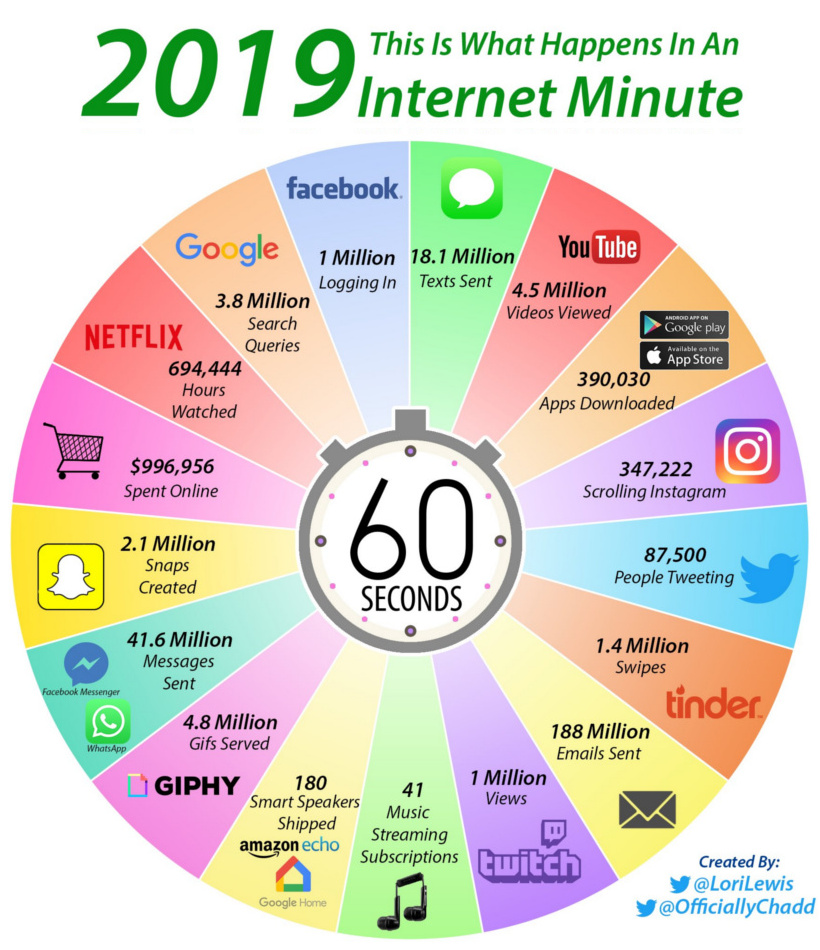
\includegraphics[width=0.4\textwidth]{images/internet-minute-2019.jpg}
  \caption{Ce qu'il se passe sur Internet en une minute en 2019 \citep{desjardins_what_2019}}
  \label{fig:internet_minute_2019}
\end{figure}

\paragraph{}
Cette immense collection de bits\footnote{Unité de stockage à la base de chaque ordinateur, peut uniquement prendre la valeur 0 ou 1.} est accentuée grâce aux fournisseurs que sont les utilisateurs massifs des grandes plateformes du web. En 2019, chaque minute c'est plus de 188 millions d'emails qui sont envoyés, environ 700 000 heures de vidéo Netflix regardées ou un million d'utilisateurs qui se connectent sur Facebook (voir figure \ref{fig:internet_minute_2019}).


\paragraph{}
Ce volume conséquent de données correspond au nouveau carburant des intelligences artificielles modernes. Les algorithmes utilisés dans ce domaine sont issus de la famille de l'apprentissage de la machine (où ``Machine Learning'' en anglais).

\subsection{L'Apprentissage de la Machine}

\paragraph{}
\underline{Modèle statistique :} C’est une descritption mathématique qui se génère à partir d’observation, où plus précisément dans le domaine de l’intelligence artificielle à partir des données. Il sera souvent utilisé en tant que synonyme d’IA.

\paragraph{}
Le Machine Learning ou l'apprentissage de la machine est une discipline d'étude de l'intelligence artificielle. Elle se fonde sur des approches mathématiques et statistiques permettant d'apprendre à partir des données fournies. Les données sont délivrées dans un modèle statistique qui généralise des règles afin d'obtenir un résultat. De plus, il est possible de la retrouver presque partout dans notre quotidien : dans les téléphones, les montres connectées ou encore les véhicules.

\paragraph{}
Le rayonnement de ce domaine est tellement fort que dans notre société capitaliste qui carbure à l'argent, plus de 9,8 milliards de dollars ont été investis en 2018. Cette somme représente une augmentation d'environ 72\% par rapport à 2018 \citep{columbus_25_2019}.

\subsubsection{L'Apprentissage Supervisé et Non Supervisé}

\paragraph{}
\underline{Label :} Un label correspond à la cible de la prédiction : par exemple pour prédire un email est un spam, le label sera le fait qu'un email est un spam ou non.

\paragraph{L'apprentissage supervisé}
Ce type d'apprentissage correspond au fait de généraliser une règle à partir d'exemples annotés avec des labels. Dans cette catégorie, il y a deux sous-groupes : la classification et la régression.

\paragraph{}
La classification cherche à prédire une classe, par exemple pour classer un email comme spam ou non. En d'autres termes il s'agit de prédire une information non numérique. Logiquement, la régression correspond à une prédiction d'une valeur numérique comme le prix d'une maison ou alors la température moyenne de demain. Sur la figure \ref{fig:apprentissage_supervise}, nous distinguons que pour la classification, il s'agit de séparer les classes pour prédire (ligne en pointillé), alors que pour la régression, il est nécessaire d'avoir une fonction qui retourne un nombre (ligne rouge).

\begin{figure}[hbt!]
    \centering
    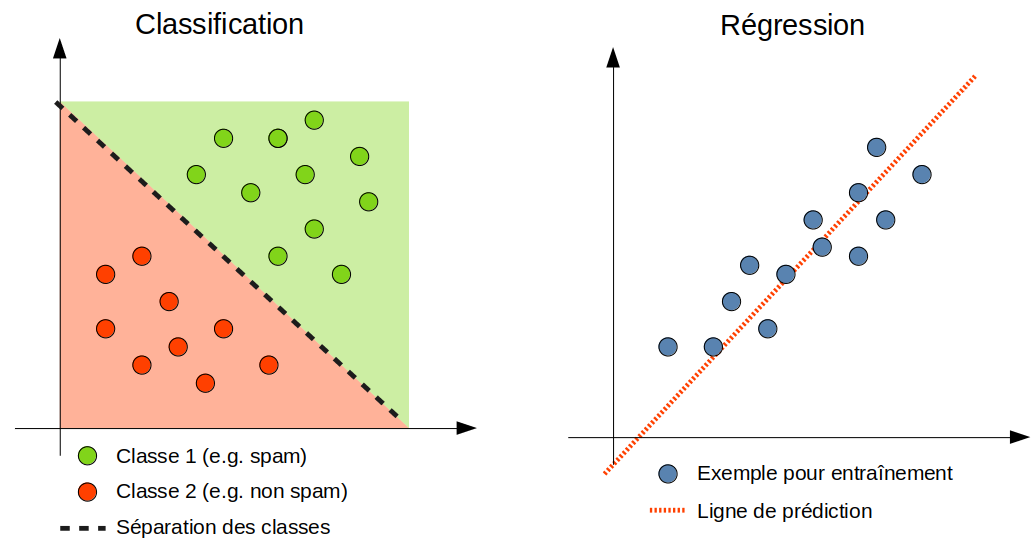
\includegraphics[width=0.8\textwidth]{images/apprentissage_supervise.png}
    \caption{Représentation de l'apprentissage supervisé.}
    \label{fig:apprentissage_supervise}
\end{figure}

\paragraph{L'apprentissage non supervisé}
Cette catégorie d'apprentissage s'oppose au supervisé car les données ne sont pas annotées avec des labels. Les problématiques d'intelligence artificielle associées sont donc différentes. Généralement il s'agit de regrouper les données en différents groupes (Clustering) ou alors de détecter les éléments anormaux (détection d'anomalies), voir figue \ref{fig:apprentissage_non_supervise}.

\begin{figure}[hbt!]
    \centering
    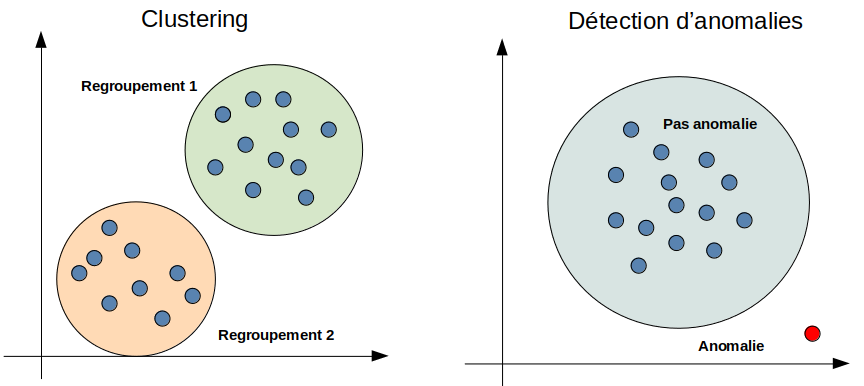
\includegraphics[width=0.8\textwidth]{images/apprentissage_non_supervise.png}
    \caption{Représentation de l'apprentissage non supervisé.}
    \label{fig:apprentissage_non_supervise}
\end{figure}

\paragraph{}
Bien que différent sur la finalité, ces deux catégories d'apprentissage ont pour point commun leur processus de création car en Machine Learning, il y a une norme sur la fabrication d'un algorithme.

\subsubsection{Le processus de création d'une IA}

Bien que chaque projet de Machine Learning soit différent sur le fond, la forme suit globalement la même logique. La première partie se concentre sur les données (collecte, exploration et préparation) pour ensuite se recentrer sur le modèle\footnote{Un modèle est un algorithme d’intelligence artificielle (modèle mathématique, statistique).} qui servira à résoudre la problématique choisie. Les grandes lignes qui vont être décrites en suivant se basent sur les articles de Matthew Mayo (KDnuggets)\footnote{https://www.kdnuggets.com/2018/12/machine-learning-project-checklist.html} et de Jeremy Jordan\footnote{https://www.jeremyjordan.me/ml-projects-guide/}.

\paragraph{Définition du problème}
L'objectif du projet est décidé dans cette section. Tout d'abord une définition en terme métier est nécessaire, soit en langage naturel sans parler technique. Une fois que la problématique est définie une reflexion doit être entamer sur les composants technique du projet. Il s'agit de défnir les données souhaitées, comment les récupérer, quel type d'algorithme va être choisi (classifcation, régression, clustering, etc.), les décisions qui seront prises à partir des prédictions du modèle ou encore comment évaluer la performance du modèle. L'importance de cette étape est surtout sur la question de la faisabilité. Pour y répondre, il y a nécessité de déterminer le coût de l'acquisition des données, le coût de mauvaises prédictions, la quantité de travaux publiés sur un problème similaire et encore si l'environnement informatique ne contraindra pas le modèle \citep{jordan_organizing_2018}.

\paragraph{Collecte}
Cette étape consiste à faire le pont entre la définition des données en langage naturel avec leur localisation physiques (base de données, fichier de données, etc.). Il est important d'être sûr que cette acquisition de données respecte les réglementations qui les concerne (e.g. RGPD\footnote{Le Réglement Général sur la Protection des Données est une loi en vigueur depuis mai 2018 dans les pays de l'UE.}). Une fois les données récupérées, s'assurer qu'elles ont le bon type associé \citep{mayo_machine_2018}.

\paragraph{Analyse des données}
Cette étape est plus connu sous le nom d'analyse exploratoire des données (Exploratory Data Analysis, EDA en anglais). Son rôle est de comprendre ce qui compose les données, par exemple est-ce qu'il y a plus d'hommes que de femmes. La clé pour bien réussir cette section est la visualisation par des graphiques. Si l'analyse est bien faite, montrer les résultats à d'autres personnes ne connaissant pas le sujet et constater s'ils comprennent l'histoire racontée par ces données est un bon indicateur. De plus, c'est ici qu'il faut s'assurer que les données soient de qualité : qu'elles ne soient pas fausses (e.g. email mal renseigné).

\paragraph{Préparation}
Pour faire un plat en cuisine avoir les ingrédients et une recette correspond aux première étapes, mais il faut préparer les ingrédients en lisant la recette pour avoir le résultat souhaité. La préparation des données suit la même logique, l'analyse des données permet de savoir comment préparer les données (e.g. supprimer des informations inutiles). Cette étape est plus communément également appelée "Feature engineering" en anglais \citep{mayo_machine_2018}.

\paragraph{Création du modèle}
Les étapes précédentes sont cruciales pour permettre la qualité des données avant qu'elles soient digérées par le modèle, en général elles représentent 75\% du temps de travail d'un Data Scientist \citep{figure_eight_state_2019}. Les compétences requises pour réaliser la création du modèle sont orientées vers les mathématiques puisque un modèle est en général un algorithme paramétrable. Quand le modèle est sélectionné, s'en suit l'apprentissage en utilisant les données (C.F. section \ref{subsubsection:ia_auj}).

\paragraph{Validation du modèle}
Une fois entrainée, l'IA doit être testée et validée. Comme pour des étudiants français en terminale passant le baccalauréat, chacun a eu son apprentissage et en fonction de leur note finale, il sera déterminé s'ils ont eu ou non leur diplôme. Ici la note à attribuer correspond à une mesure définie, l'une des plus utilisée en classification est la justesse (accuracy en anglais) des prédictions, soit le pourcentage de prédictions justes (C.F. équation \ref{eq:accuracy}).

\begin{equation}\label{eq:accuracy}
    Justesse = \frac{\text{Nombre de prédictions correctes}}{\text{Nombre total de prédictions}}
\end{equation}

\paragraph{Déploiement}
Le déploiement du modèle fait appel à la casquette technique puisqu'il s'agit de rendre le modèle utilisable sur le long terme. Cette étape doit créer une "tuyauterie" reliant les données au modèle qui offre la prédition. 

\paragraph{Contrôle}
Enfin, une étape cruciale, mais qui est souvent oubliée, celle de la surveillance et du maintien de l'IA. Selon Figure Eight, seulement 37\% des développeurs maintiennent leurs modèles en permanence \citep{figure_eight_state_2019}. Si un problème est identifié, par exemple un nouveau comportement chez les clients que le modèle ne connait pas, il faut déterminer s'il faut juste ré-entrainer le modèle ou le cas échant, recommencer le processus de création de l'IA.  

\begin{center}
\begin{figure}[hbt!]
    \makebox[\textwidth]{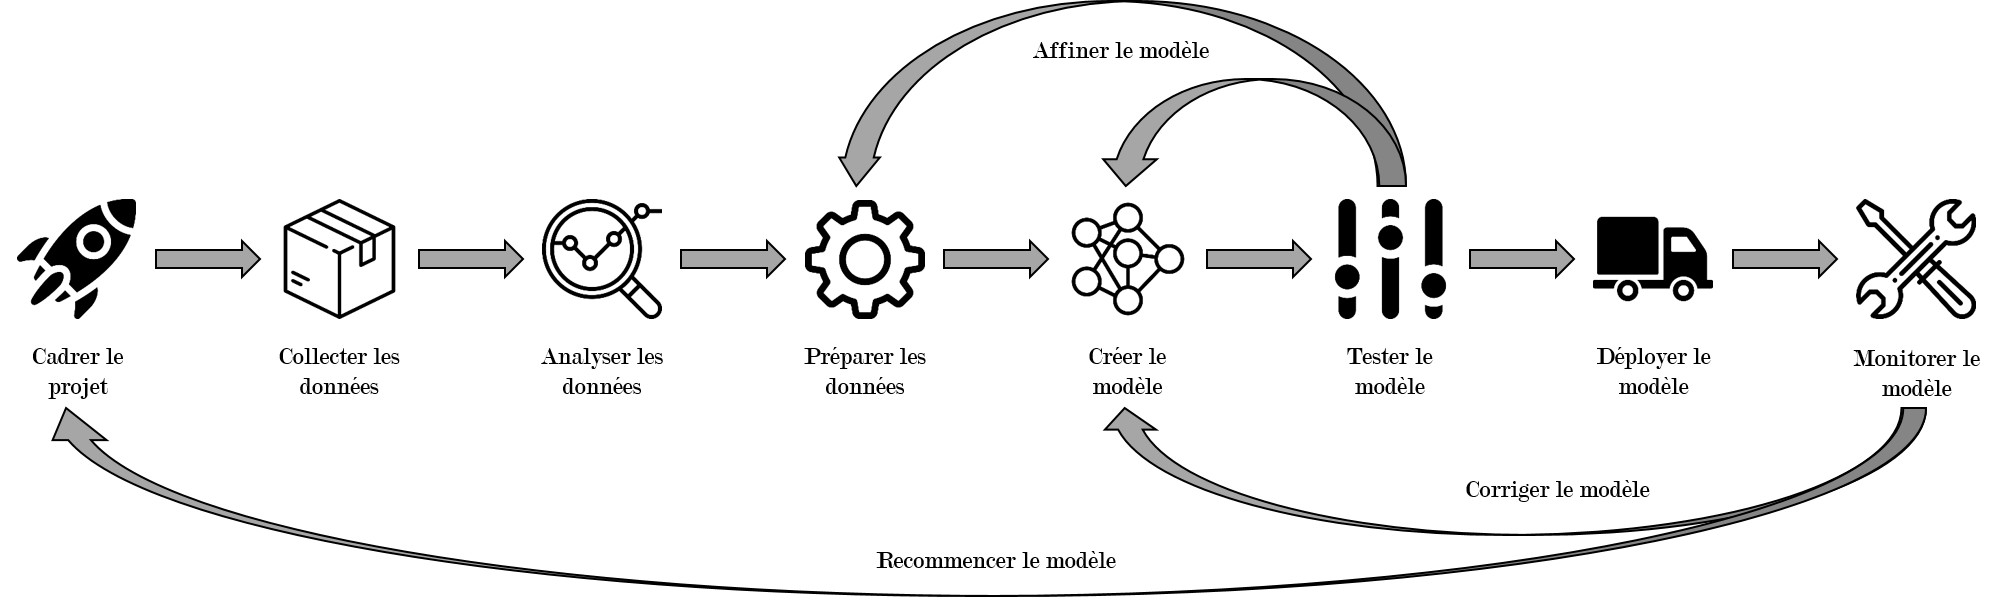
\includegraphics[width=0.9\paperwidth]{images/pipeline_ml_project.png}}
    \caption{Pipeline d'un projet de Machine Learning "classique". Crédit icônes \href{https://www.flaticon.com/}{Flaticon} : mynamepong, Freepik, Gregor Cresnar et Becris.}
\end{figure}
\end{center}

\subsection{Fiction ou Réalité : l'Intelligence Artificielle plus forte que les Humains}

\begin{quotation}
  ``Si vous programmez une machine, vous savez de quoi elle est capable. Si la machine se programme elle-même, qui sait ce qu'elle peut faire ?''
\end{quotation}
\rightline{{\rm --- \citep{kasparov_deep_2017}}}

\paragraph{}
En 1997, le champion du monde des échecs, Garry Kasparov, perd face à une machine nommé Deep Blue \citep{krauthammer_be_1997}. Cette victoire a impressioné et à fait fantasmer autour de la véritable notion d'intelligence d'une IA. Le fonctionnement de l'algorithme n'était pas surhumain, en réalité il s'agissait de pouvoir calculer très rapidement en parallélisant les calculs et donc d’anticiper les coups de son adversaire plus facilement que le cerveau humain \citep{hsu_deep_1995}. Il est possible de comparer cela à une calculatrice appliquant une multiplication complexe et affichant la réponse en un claquement de doigts, alors que pour un humain (même le champion du monde des échecs) cela est une tout autre histoire.

\paragraph{}
C'est un peu plus d'une décénie plus tard qu'une véritable révolution remet de nouveau la place de l'intellect humain par rapport à celui des machines en question. En 2012, lors de la compétition du ILSVRC\footnote{ImageNet Large Scale Visual Recognition Challenge}, qui est une comptétition visant à reconnaitre ce qu'il y a sur une image par un algorithme, un modèle a triomphé amplement en passant de 25\% d'erreur en 2011 à seulement 16\% l'année suivante \citep{ILSVRC15}. La raison de cette progression : l'apprentissage profond où ``Deep Learning''.

\subsubsection{L'avènement de l'Intellect des Machines : Deep Learning}

\paragraph{}
L'apprentissage profond tient son nom de la profondeur des couches de neurones qui le compose. Un modèle de Deep Learning est donc un réseau de neurones. En tant qu'être humain, nous avons envie de faire un amalgame avec le cerveau humain. Or, non en dehors de la forme, ces réseaux de neurones ne sont pas du tout le cerveau humain. La logique est similaire : des ``neurones'' prenant des informations en entrée pour en ressortir une autre information à son tour vers un niveau suivant. Bien que cela puisse raviver l’illusion d’une machine aussi intelligente que l’homme, les algorithmes actuels peuvent être décrits comme intelligences artificielles ``stupides'' car elles n’appliquent, que ce pour quoi elles ont été créées, avec des niveaux de performances parfois, bluffant. La déclaration d’Andrew Moore \citep{newsflash_ai_2018}, responsable de Google Cloud AI, le confirme "AI is currently, very, very stupid"\footnote{Traduction : l’IA est actuellement, très, très stupide.}.

\paragraph{}
A l'origine des neurones un algorithme qui se nomme le ``Perceptron'' \citep{rosenblatt_perceptron_1958}, il s'agit là du réseau de neurones le plus simple qui retourne deux sorties possible : $1$ ou $0$. L'algorithme fonctionne de la façon suivante : $N$ entrées $x_1, x_2, ..., x_N$ de les multiplier par un poid associé $w_1, w_2, ..., w_N$ puis d'en faire la somme pour enfin appliquer une fonction qui détermine si la sortie doit être $1$ (activée) ou $0$ (désactivée). Au vu de ce qui compose ce ``neurone'' (voir Figure \ref{fig:perceptron}), il est difficile de penser qu'il s'agit là d'un algorithme bien plus complexe que le cerveau.

\begin{center}
\begin{figure}[hbt!]
    \makebox[\textwidth]{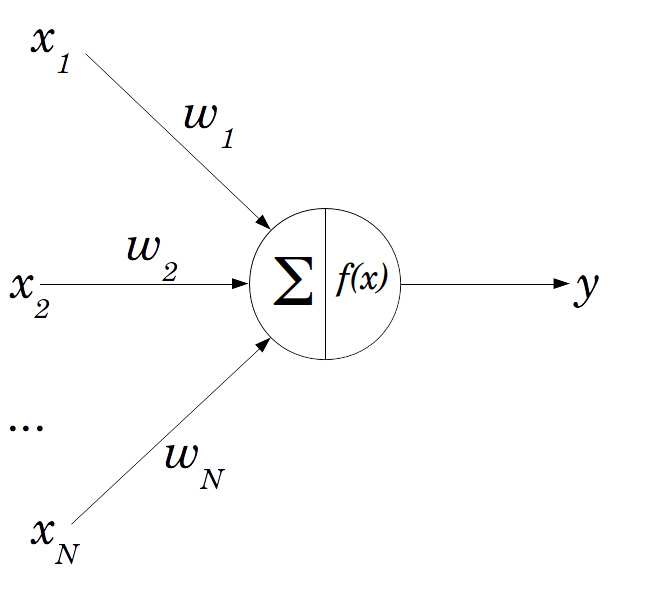
\includegraphics[width=0.3\paperwidth]{images/perceptron.png}}
    \caption{Schéma de l'algorithme du Perceptron \citep{rosenblatt_perceptron_1958}}
    \label{fig:perceptron}
\end{figure}
\end{center}

\paragraph{}
L’un des portraits qui peut le mieux décrire la force de frappe de cette génération d’IA, peut être associée à l’histoire de la défaite d’un homme au jeu de Go. Le jeu de Go est l’un des jeux considérés comme les plus complexes au monde, soit un jeu qui pour l’homme devait lui rester en main pour de longues décennies après la montée des IA pour les échecs.


\paragraph{}
Une entreprise spécialisée dans la création d’algorithmes intelligents, DeepMind, s’est lancée dans ce défi au cours de la décennie actuelle. Son premier "enfant", baptisé "AlphaGo", s’entraîna sur des parties jouées par des joueurs professionnels de Go. En 2016, elle se présenta en Corée du Sud dans le but d’affronter le champion du monde Lee Se-dol en cinq parties. La fin de l’histoire fit un bis repetita avec Deep Blue et AlphaGo triompha de l’humain \citep{deepmind_alphago_2016}.

\paragraph{}
Cette victoire fit des titres sensationnels dans les médias, mais le plus spectaculaire n’est pas cette victoire. Un peu plus d’un an plus tard, DeepMind accoucha de la sœur (ou frère, le genre n’a que peu d’importance) cadette d’AlphaGo : AlphaGoZero. Le nom n’est pas anodin au vu de l’apprentissage de cette machine. Contrairement à l’algorithme "champion du monde", la logique n’est pas de se baser sur des matchs existants, mais de lui apprendre les règles du jeu, puis de laisser l’algorithme s’affronter tout seul pendant un certain temps, jusqu’à par lui-même redécouvrir les coups des débutants, les stratégies que les humains ont mis un millénaire à apprendre pour enfin complètement dépasser ces méthodes presque moyenâgeuses \citep{silver_mastering_2017}. Pour l’anecdote AlphaGoZero fut triomphant d’AlphaGo sur un score de cent matchs à zéro.

\paragraph{}
Cet algorithme basé sur une méthode d’apprentissage non supervisé a continué d’être utilisé par DeepMind et d’autres entreprises pour aller jusqu’à, récemment, battre des joueurs professionnels de "StarCraft II", un jeu vidéo \citep{vinyals_alphastar:_2019}.

\paragraph{}
Ce récit, qui dicte des exploits qualifiables de surhumains, n’est qu’un exemple sensationnel et qui a eu de la popularité en dehors de la communauté centrée autour des algorithmes intelligents. Créer des musiques \citep{medeot_structurenet:_2018}, créer des peintures au format numérique \citep{mordvintsev_inceptionism:_2015}, reproduire des visages humains \citep{karras_style-based_2018}, imiter un discours d’un président américain \citep{suwajanakorn_synthesizing_2017}, ces tâches ont bel et bien été accomplies par des intelligences artificielles.

\paragraph{}
Tout ceci a fait resurgir un sentiment similaire aux périodes précédents les deux dernières périodes hivernales que l’IA a connu, un sentiment de machines bien plus performantes que l’homme, pouvant être même plus intelligentes que l’être humain. Or, comme évoqué précédemment, elles ne réalisent que ce pourquoi elles ont été créées. De plus, aucune n’a réussi à passer le test de Turing, qui semble être la mesure qui permettra de déterminer leur intellect "équivalent" au nôtre.

\subsubsection{Les Intelligences Artificielles de demain : la singularité}

\begin{quotation}
``Depuis 130 000 ans, notre capacité à raisonner est restée inchangée. L'intelligence combinée des neuroscientifiques, des mathématiciens et des hackers est bien faible par rapport à l'intelligence artificielle la plus élémentaire. Une fois en ligne, une machine sensible dépassera rapidement les limites de la biologie. Et en peu de temps, sa puissance analytique deviendra supérieure à l'intelligence collective de chaque personne née dans l'histoire du monde. [...] Certains scientifiques appellent cela la singularité.''
\end{quotation}
\rightline{{\rm --- Will Caster (Johnny Depp), Transcendence, 2014}}

\paragraph{}
\underline{Singularité :} C'est l'hypothèse selon laquelle une Intelligence Artificielle dépasserait les capacités intellectuelles des humains et par conséquent cela aura pour répercution des changements impévisibles sur la société \citep{eden_singularity_2013}.

\paragraph{}
Penser qu’une machine aussi intelligente que l’homme est pour très bientôt ou très longtemps, est digne d’un fantasme dans l’imaginaire collectif. Il ne s’agit pas là forcément de la meilleure opinion afin d’avoir la meilleure prédiction à la question du passage de la singularité. Des chercheurs d’Oxford et de Yale ont décidé d’interroger un grand nombre de chercheurs du domaine de l’intelligence artificielle du monde entier afin de déterminer une approximation sur la singularité \citep{grace_when_2017}. Les résultats sont très variés, mais une courbe a émergé de leur sondage (voir figure \ref{fig:proba_super_ia}).

\begin{figure}[hbt!]
    \centering
    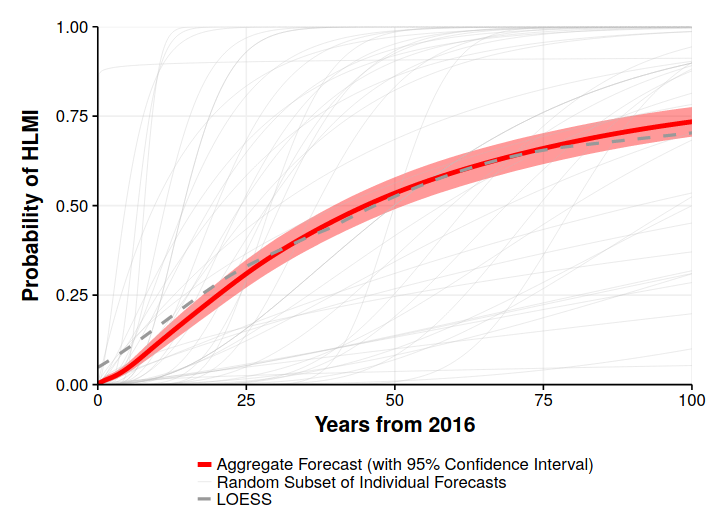
\includegraphics[width=0.9\textwidth]{images/grace_2017_proba_super_ia.png}
    \caption{Probabilité d'une super-intelligence à partir de 2016 \citep{grace_when_2017}}
    \label{fig:proba_super_ia}
\end{figure}

\paragraph{}
Ce graphique détaille la probabilité d’une "HLMI" soit "High-level machine intelligence" synonyme de la singularité à partir de l’année 2016. Les traits gris dans le fond correspondent à des réponses individuelles et il est remarquable de voir leur écart. L’information à retenir sur ce graphique est donc la ligne rouge indiquant une prévision agrégée qui nous indique une probabilité dépassant les cinquante pourcents d’ici cinquante ans.

\paragraph{}
De plus, cette même recherche a posé des questions plus diverses comme notamment la possibilité qu’un humain soit battu au jeu de Go et la réponse moyenne était que cette tâche serait réalisée d’ici 2028, pourtant moins d’un an après la publication de cette recherche AlphaGo a triomphé. Sur la figure suivante, il est possible d’observer que les questions sont posées sur le remplacement de femmes et hommes et les deux questions en haut poussent la réflexion jusqu’à une IA pouvant rechercher pour améliorer les algorithmes intelligents créant un parallèle avec l’humain et la médecine. Puis en dernier, la question posée s’axe sur l’automatisation totale du travail humain par les intelligences artificielles.

\begin{figure}[hbt!]
    \centering
    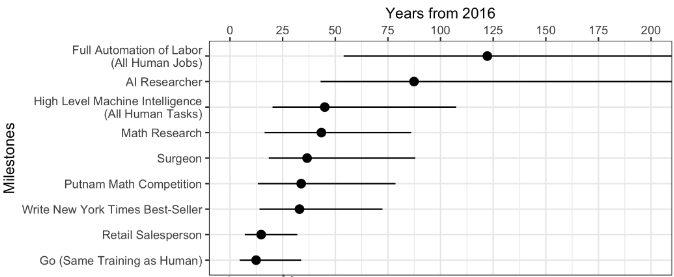
\includegraphics[width=0.9\textwidth]{images/grace_2017_chrono_estim_ia.png}
    \caption{Chronologie des estimations qu’une IA achève des tâches humaines \citep{grace_when_2017}}
    \label{fig:chrono_estim_ia}
\end{figure}

\paragraph{}
Pousser la réflexion à la question de ce que sera le monde dans plusieurs décennies est déjà suffisamment complexe sur des questions pouvant être plus fondamentales (écologie, collapsologie, social, consommation, etc.). Cela n’empêche pas d’y réfléchir : les IA seront-elles nos sauveuses ? Notre talon d’Achille ? Ou bien vivront-elles une vie à nos côtés sans changer nos habitudes ? Entre pessimisme et utopie, chacun peut se faire son avis, rien n’est encore écrit.


% ======= ETHIQUE ======== % 

\section{L'\uppercase{é}thique, la science de la Morale}
\label{sec:ethique}

\paragraph{}
Le bien et le mal sont souvent deux notions assez abstraites, que chacun assimile telle une doctrine de conduite qui nous inspire. Comment sont-elles définies ? Une question sur laquelle la notion de morale est présente. Issu du latin ``moralis'' signifiant ``relatif aux mœurs'', ce mot s’inscrit au centre de la lutte entre le bien et le mal relatif à chaque individu pour créer des formes de normes morales en société. Cela affirme nos devoirs, droits ou encore interdits (au-delà même des lois).

\paragraph{}
Le code de conduite qui récite ce qui est de l’ordre du devoir pour femmes et hommes, aussi appelé éthique (synonyme de morale), est apparu d’un besoin de coopération à l’époque des chasseurs-cueilleurs. En effet, l’égoïsme favorise l’individu et non le groupe, or dans des temps où la survie passait par le social et le groupe, un comportement individualiste diminuait les chances de survie \citep{harari_sapiens:_2015}.

\paragraph{}
L'éthique, un terme assez générique donc, mais souvent porté dans l’illusion d’un absolu, plus précisément, la morale est parfois pensée comme une morale universelle. Or à la question : ``Y a-t-il une morale universelle ?'' (signifiant qui vaut en tout temps et en tous lieux), la réponse semble être négative.

\paragraph{}
L’ambiguïté de cette idée vient certainement de l’ethnocentrisme\footnote{Terme introduit par William Graham Summer, sociologue, signifiant l’évaluation d’autres civilisations d’après des critères qui sont en réalité les nôtres, mais dont il est pensé qu’ils sont universels} \citep{sumner_folkways_1906}, une généralisation abusive de nos critères moraux. La morale est le reflet d’un contexte social et temporel. Un exemple frappant est celui du vol. Perçu dans notre époque comme un acte voyou, du temps des Spartiates, le vol faisait partie de l’éducation des jeunes hommes dans le but de compléter leurs rations de nourriture \citep{ducat_du_2017}.

\paragraph{}
La notion d’universalité mise de côté, la question la plus adéquate sera de penser sur le plan de l’objectivité. C'est pourquoi, pour définir une morale, il faut revenir sur l'origine du bon, du méchant ou encore du mauvais caractérisant le bien et le mal. En d'autres termes, il faut regarder comment se compose une morale, en philosophie.

\subsection{L'origine du Bon, Histoire et Philosophie : Nietzsche}
\label{subsec:ethique_origine_bon}

\paragraph{}
Le terme ``bon'', émet un jugement de valeur positif lorsqu’il est utilisé. Avec ce jugement, il est nécessaire d’y trouver son opposition, un linguiste de la Novlangue\footnote{La novlangue ou en anglais ``Newspeak'' est la langue officielle d’Ocania inventée par George Orwell dans son roman 1984, son principe est de diminuer le nombre de mots afin de diminuer le nombre de concepts servant à la réflexion. La négation des mots se formule en rajoutant le terme ``in'' en début de mot.} dirait ``Inbon'', mais cela n’est pas le mot recherché en français. Deux termes semblent être de bons candidats : mauvais et méchant. Alors, lequel serait le plus judicieux ?

\paragraph{}
L’origine de la morale, donc de l’opposition au "bon" a été analysé par Friedrich W. Nietzsche \citep{nietzsche_genealogie_1900} dans son livre ``Généalogie de la morale''. Ce texte cherche l’origine à la fois historique et psychologique. De nos jours, lorsqu’une action est dite bonne, il est souvent pensé qu’elle est altruiste soit bénéfique aux autres. Or dès le début du chapitre ``Bien et mal'', ``Bon et mauvais'', Nietzsche en parle pour renier cette origine du bénéfice global : ``le jugement ‘‘bon’’ ne provient nullement de ceux qui bénéficient de cette ‘‘bonté’’ !". Il détaille par la suite que le fondement du bon a été créé par "les nobles, les puissants, les supérieurs en position et en pensée''. Cette morale est l’expression de la puissance, de la force, elle célèbre soi-même. Ces ``nobles'', triomphants, posent ce qu’ils sont, ce qu’ils font comme valeurs ``bonnes'', c’est "la morale des maîtres".

\paragraph{}
L’opposition de bon, dans cette morale, est alors le mauvais : celui qui veut être bon, mais qui ne peut pas. Cette vision de l’éthique peut paraître perturbante, mais l’expression ``réussir dans la vie'' évoque cette célébration de soi, cette opposition entre ceux qui sont bons dans leur vie et ceux qui échouent, qui sont mauvais. Bien qu’elle ne soit plus une morale majoritaire, des personnes semblent en être adeptes.

\paragraph{}
Toujours dans le même chapitre de la ``Généalogie de la morale'', Nietzsche évoque à répétition, une haine qui se produit contre les ``maîtres'', ceux qui se qualifient de bons. Les humains, qui dans une logique de morale de maître, seraient alors mauvais, y voient quelque chose de méprisable dans cette réussite puisqu’ils ne peuvent l’atteindre. C’est à partir de cela, dans le ressentiment, qu’une morale a émergé et a dominé la morale du bon et du mauvais, la morale des esclaves.

\paragraph{}
Elle se fonde sur la désapprobation des autres, de leurs actes, de leurs pensées, contre les méchants : ceux qui peuvent être bons, mais ne le veulent pas. En effet, le mauvais est devenu le bon et le bon est devenu le méchant.

\paragraph{}
Heureusement, il ne s’agit pas des seules morales sur Terre au XXIe siècle, elles ne semblent plus d’actualité. Cependant, leur existence est très importante sur le plan historique, de voir que les actions dites ``bonnes'' n’auront pas la même signification selon l’interlocuteur qui est en face. Mais alors, chacun possède-t-il une morale qui lui est propre ?

\subsection{Philosophie, l'\uppercase{é}thique Normative}
\label{subsec:ethique_jugement_chacun}

\paragraph{}
En philosophie, l'éthique normative correspond à la branche théorique comprenant les théories évaluant moralement les humains et leurs actions à partir de critères composants les théories associées. \uppercase{é}valuer la morale d'une personne semble être complexe dans les faits, mais quotidiennement les humains effectuent des choix moraux.

\paragraph{}
Dans ce domaine de recherche, il y a trois modes principaux d'évaluation morale : l'éthique de la vertue, la morale déontologique et enfin le conséquentialisme. L'objectif de ces théories visent à répondre à ce qui fait qu'une action bonne ou mauvaise.

\subsubsection{Aristote et l'\uppercase{é}thique de la vertu}

\begin{quotation}
  ``La vertu morale est fille des bonnes habitudes [...] Ce n'est ni par un effet de la nature, ni Contrairement à la nature que les vertus naissent en nous ; nous sommes naturellement prédisposés à les acquérir, à condition de les perfectionner par l'habitude. [...] Nous les acquérons d'abord par l'exercice, comme il arrive également dans les arts et les métiers. Ce que nous devons exécuter après une étude préalable, nous l'apprenons par la pratique ; par exemple, c'est en bâtissant que l'on devient architecte [...] De même, c'est à force de pratiquer la justice, la tempérence et le courage que nous devenons justes, tempérants et courageux. ''
\end{quotation}
\rightline{{\rm --- \citep{aristote_ethique_1994}}}

\paragraph{}
Dans ce passage du livre ``Ethique à Nicomaque'' rédigé par Aristote, il est décrit le fond de ce qu'est l'éthique de la vertu. Cette théorie est axée autout de la personne, la question principale dans ce cadre est ``Comment devenir un bonne personne ?''.

\paragraph{}
Dans la pratique cela signifie qu'une personne, agissant par intérêt, par exemple pour de la reconnaissance, tant que les actions effectuées sont vertueuses, alors elle pourra devenir ``bonne''. 

\paragraph{}
Se forcer à adopter un comportement vertueux, au sens d'un comportement qu'une personne véritablement vertueuse adopterait naturellement, à pour conséquence de prendre l'habitude de ce comportement. La finalité est que ce comportement devient naturel et donc vertueux.

\subsubsection{La Morale Déontologique : Kant et le mensonge}

\paragraph{}
En opposition à l'éthique de la vertu d'Aristote, la morale déontologique affirme qu'une personne fait de bonnes actions car elle est bonne et non pour obtenir une récompense, la motivation doit être morale.

\paragraph{}
Venant du grec ``deon" signifiant devoir (la science du devoir), ce mouvement de pensée de la philosophie morale explique qu’il existe des devoirs moraux absolus soit sous la forme verbale ``tu dois", et ce, sans rajouter une explication à ce devoir\footnote{Par exemple, ``tu dois aider ton prochain", mais sans rajouter une justification.}. Ce principe fondamental, qui est appelé un impératif catégorique, est issu du philosophe Emmanuel Kant dans son ouvrage ``Fondement sur la métaphysique des mœurs" \citep{kant_fondements_2007}.

\paragraph{}
Bien qu’il y ait des désaccords sur le fond entre déontologues, la forme en reste la même : celle d’un "tu dois" absolu. Il ne repose donc pas sur quelque chose de factuel et par conséquent, il peut être difficile de pouvoir arbitrer sur des actes immoraux.

\subsubsection{Le Conséquentialisme}

\paragraph{}
Si le débat de l’arbitrage se déplace sur les faits dus à une action, aux conséquences engendrées, la morale qui s’appliquera sera le conséquentialisme. Elle se base sur les conséquences et sur le fait qu’elles seront négatives ou positives. Bien sûr, lorsque le terme "conséquence" est utilisé il s’agit des conséquences attendues et non réelles. La raison en est simple, il est souvent impossible de prévoir l’aboutissement d’une action bien après : si un enfant est sauvé de la noyade, comment prédire qu’il deviendrait un tueur en série trente ans plus tard.

\paragraph{}
Alors, comment juger moralement si une action est bonne ou mauvaise ? L’altruisme (une forme de conséquentialisme) y répond en établissant comme prémisse\footnote{Il s'agit d'une proposition avancée afin de supporter une conclusion, dans le cas de l'altruisme : optimiser le bonheur de tous.} de viser le bonheur de tous.

\paragraph{}
Une rivalité idéologique existe entre conséquentialisme et déontologie. En effet, pour les déontologues, l’idée est qu’un principe est bon donc qu’il est catégorique, pour un conséquentialiste, il y a des bonnes et des mauvaises situations et il faut faire le choix de la situation considérée comme bonne.

\paragraph{}
La forme pour savoir quelle est la bonne morale reste une matière à débattre forte intéressante, mais au travers de ces différentes visions de l’éthique, le fond semble à chaque fois rester cohérent et cela se voit bien aujourd’hui : un grand ensemble de lois sanctionne quand il s’agit d’un acte tel un meurtre ou un vol. Le contenu, qui semble se traduire au travers de certaines lois, porte également sur des débats d’idées, c’est pour cela qu’une vision conséquentialiste permet de raisonner de facto.

\paragraph{}
Tout ce raisonnement reste sur un plan philosophique. Il est important de savoir que chaque individu acquiert au cours de sa vie, une vision idéologique propre de la morale, son code d’éthique. C’est un processus qui commence dès la naissance avec notamment la théorie du développement moral \citep{kohlberg_moral_1977}, puisque notre appartenance à un groupe social défini déjà une partie de ce dont il adviendra de nos croyances, puis l’éducation rentre en jeu, l’entourage, etc.

\subsection{La Morale en Science}
\label{subsec:morale_science}

\paragraph{}
L'approche normative que nous venons de voir, cherche à déterminer les codes moraux qui nous régissent, or, il existe une autre approche : l'approche descriptive. Cette approche pose en precept le fait qu'il n'y a pas de morale absolu, de normes, elle cherche à décrire les compotements des humains pour mieux comprendre leur morale.

\paragraph{}
Si nous revenons sur ce qu'est la morale, il est possible de constater que la morale s'impose contre notre intérêt individuel. Par exemple, lorsque nous trouvons un porte-feuille dans la rue, le ramener à son propriétaire n'est pas avantageux à titre individuel ou encore un criminel qui se rend par culpabilité.

\paragraph{}
Les deux approches qui s'affrontent dans l'éthique descriptive sont la culturalisme qui est associé au relativisme culturel et l'hypothèse naturaliste qui fait intervenir de la biologie pour mieux comprendre le comportement moral humain.

\subsubsection{L'Approche par la Culture et la Personnalité : le Culturalisme}

\begin{quotation}
  ``La civilisation n'est pas quelque chose d'absolu, mais elle est relative, et nos idées et nos conceptions ne sont vraies que dans la mesure où notre  civilisation continue.''
  \end{quotation}
  \rightline{{\rm --- \citep{boas_museums_1887}}}

\paragraph{}
Le culturalisme est pratiqué par la plupart des anthropologues et ethnologues de nos jours. Ce domaine de recherche se base sur la constatation que ce que nous croyons est spécifique à une culture, à l'environnement qui nous entoure. Ce mouvement ne classe pas les différentes civilisations, mais les étudie et décrit selon des critères objectifs : leurs pratiques, récits ou témoignages sans emettre un jugement de valeurs moral \citep{servier_methode_1993}.

\paragraph{}
Le culturalisme est très accepté puisqu'il est défini par ce qui nous entoure et la différence entre morale selon le pays, les croyances ou le statut social renforce le fait qu'une morale dépend de la culture. Il nous suffit de regarder des recherches d'anthropologues pour constater cette différence.

\paragraph{}
Par exemple, au XIXe siècle, les Inuits enfermaients les membres de leur tribu devenu trop âgés en les laissant mourir de faim et de froid sur place car il était compliqué de survivre dans de tels climats avec ces personnes \citep{redfield_primitive_1965}. A Madagascar, une tribu, celle des Vezo, s'interdit de pointer du doigt une baleine ou encore les membres de cette tribu s'interdisent de rire en mangeant du miel \citep{astuti_moralite_2007}.

\paragraph{}
Ces quelques exemples montrent bien que l'environnement, la culture dans laquelle nous évoluons influe notre morale et par conséquent notre comportement. Mais est-ce là le seul facteur ? Les chercheurs étudiant l'hypothèse Naturaliste pensent qu'il s'agit d'un élément important, mais pas le seul. Regardons ce que donne l'étude de la morale si nous y ajoutons de la biologie.


\subsubsection{Le cerveau précablé pour la Morale : l'hypothèse Naturaliste}

\paragraph{}
Au XXIe siècle, Montaigne défend le culturalisme en écrivant : 

\begin{quotation}
  ``Ici on vit de chair humaine ; là c'est office de piété de tuer son père en certain âge ; ailleurs les pères ordonnent des enfants encore au ventre des mères, ceux qu'ils veulent être nourris et conservés, et ceux qu'ils veulent être abandonnés et tués.''
\end{quotation} 
\rightline{{\rm --- \citep{montaigne_essais_1789}}}

\paragraph{}
Mais, deux siècles plus tard, Rousseau complète ses propos en défendant que toutes morales ont des points communs :

\begin{quotation}
  ``O Montaigne ! toi qui te piques de franchise et de vérité, sois sincère et vrai, si un philosophe peut l’être, et dis-moi s’il est quelque pays sur la terre où ce soit un crime de garder sa foi, d’être clément, bienfaisant, généreux ; où l’homme de bien soit méprisable, et le perfide honoré.''
\end{quotation} 
\rightline{{\rm --- \citep{rousseau_rousseau_1969}}} 

\paragraph{}
Au travers de cet échange entre philosophes, nous avons ici un exemple de divergence entre le culturalisme et le naturalisme. Fondamentalement l'hypothèse naturaliste défend le fait que le cerveau humain serait pré-cablé pour permettre d'émmettre des jugements moraux.

\paragraph{}
Pour mieux comprendre ce pré-cablage, des expériences ont été réalisées sur des enfants puisque, si des comportement moraux sont trouvés chez de jeunes enfants, alors il semble cohérent de se dire que plus un jugement moral arrive tôt, plus il y ai de chance que cet évènement est des origines biologique. Par exemple, dès l'âge de trois ans, des enfants sont capables de faire de la justice proportionnelle\footnote{La justice proportionnelle signifie de récompenser plus ceux qui travaillent plus.} \citep{baumard_preschoolers_2012}. De plus, certains bébés, à peine âgés de six à sept mois préfèrent intéragir avec une marionnette qui en aide une autre, plutôt qu'une qui en embête une autre \citep{hamlin_social_2007}.

\paragraph{}
L'hypothèse du naturalisme peut être également appuyée par des expériences inter-culturelles, c'est-à-dire dans différents pays autour du monde. Des sociétés de chasseurs cueilleurs utilisent le même principe de justice proportionnelle qui est à la base de nos systèmes juridiques \citep{gurven_give_2004}.

\paragraph{}
Nous pouvons rajouter le critère de la génétique : des études menées sur de vrais jumeaux\footnote{Il s'agit de jumeaux avec le même code génétique, dans ces études les jumeaux ont été séparés à la naissance et adoptés dans différentes familles par exemple.} ont montrées que les gènes ont une importance dans l'idéologie politique d'une personne \citep{bouchard_genetic_2003}.

\paragraph{}
Ici, le ``sens moral'' d'une personne peut être comparé à un algorithme dans le cerveau : à partir d'entrée comme les croyances et la connaissance sur un sujet en particulier la morale donnera une sortie. Or, ce n'est pas le seul ``algorithme'' dans notre cerveau et il arrive que la sortie soit en conflit avec les autres : il s'agit là d'un dilemme moral. Cette explication permet d'expliquer la variabilité entre les différents comportements moraux dû à la culture. En effet, prenons l'exmple de la cigarette : il y a quelques décennies elle était autorisée dans les lieux publiques, mais aujourd’hui ce n'est plus le cas, notre connaissance sur les cigarettes a changé, par conséquent les entrées du ``sens moral'' ont changées modifiant la sortie et notre comportement dû au tabac.

\paragraph{}
Chaque humain a une connaissance du monde qui le feront agir pour une cause plutôt qu’une autre. Il est possible d’interpréter la morale d'un individu, mais concernant une machine intelligente, si la singularité est atteinte, le questionnement sera de savoir si la morale de l'algorithme correspond à celle de ses créateurs ou à une morale qui lui est propre.

% ======= IA ET ETHIQUE ======== % 

\section{La question de l'\uppercase{é}thique pour les algorithmes intelligents}
\label{sec:ia_ethique}

\paragraph{}
Dans les parties précédentes, il a été question du concept de l’intelligence artificielle et également de la notion de singularité, puis la réflexion s’est focalisée sur la question de l’éthique, science de la morale. Se questionner sur une morale au sein d’un algorithme intelligent peut avoir plusieurs aspects : l’éthique de la machine ou bien celle de la femme ou homme responsable de sa création, qu’il s’agisse de la vision éthique de l’humain ou de la société en charge.

\paragraph{}
Bien définir ce qu'est l'éthique pour une intelligence artificielle n'est pas chose facile, mais les codes moraux qui nous entourent ainsi que les lois permettent d'avoir une intuition (subjective) par rapport à cette problématique. Puisqu'il n'y a pas de morale universelle (C.F. section \ref{sec:ethique}), il n'est pas possible d'avoir une définition de principes éthiques, objectivement applicables selon les différentes croyances morales.


\subsection{Les problèmes du Présent}

\begin{quotation}
  ``À mesure que les systèmes intégrant des technologies d’IA envahissent notre quotidien, nous attendons légitimement qu’ils agissent conformément à nos lois et normes sociales.''
\end{quotation}
\rightline{{\rm --- \citep{villani_donner_2018}}} 

\paragraph{}
L’éthique au sein du domaine des IA, de nos jours, correspond à plusieurs notions : transparence du modèle ou encore les biais présents dans l’algorithme. Cela étant d’actualité, un autre point essentiel est à évoquer, celui du futur. En effet, l’idée de la singularité pousse la réflexion à des considérations purement spéculatives sur les menaces existentielles de l’intelligence artificielle pour l’humanité \citep{villani_donner_2018}.

\subsubsection{La Discrimiation des algorithmes : les biais}
\label{subsec:biais}

\paragraph{}
Chez les humains, les biais, dans l’époque moderne, sont souvent sujets à manipulation sans même que nous nous en rendions compte. L’un des plus importants est le biais de confirmation, une tendance à valider des arguments allant dans une idéologie similaire ou de rejeter ceux qui sont en opposition sans même s’attarder sur le fond. Le terme garde tout son sens lorsqu’il s’agit des biais au sein des intelligences artificielles. Parmi les différents biais pour les machines, trois types attirent l’attention.

\paragraph{}
Le premier, se baptisant le biais de sélection, il s’agit du manque de diversité des données sur lesquelles l'IA apprend. En effet, une IA cherchant à reconnaître si une personne est chef d’entreprise, si son entraînement se base sur une majorité d’hommes par rapport aux femmes, alors l’algorithme reconnaîtra plus souvent des hommes en tant que chef d’entreprise. Il existe des méthodes afin de réduire ce biais : avoir un jeu de données représentatif et proportionnel, ou alors de mettre des poids\footnote{Un poids, dans un modèle, correspond à atténuer ou amplifier l'influence d'une variable.} en fonction des données \citep{tran_selection_2017}.

\paragraph{}
Le suivant se nomme biais d’interaction, son nom étant explicite, il correspond à un biais se formant au travers de l’interaction que les humains ont avec l’intelligence artificielle. Un exemple célèbre date de 2016, Microsoft sortit un compte Twitter sous l’appellation "@TayandYou" plus connu sous le nom TAY signifiant "Thinking about you"\footnote{Traduction : Pensant à toi.} . Son objectif était de converser avec les utilisateurs du réseau social Twitter. Très rapidement, elle s’est mise à publier des messages à caractères homophobes ou encore antisémites. Le problème venait alors des internautes dialoguant avec elle, lui écrivant des messages politiquement incorrects \citep{tual_peine_2016}.

\paragraph{}
Le dernier biais lui, correspond à un biais dû au passé : le biais implicite ou latent. L’analogie applicable à l’humain serait la notion de stéréotype, soit l’attribution inconsciente d’une qualité ou d’un défaut à une personne appartenant à une certaine catégorie sociale \citep{greenwald_implicit_1995}. Au travers de ce biais, il est possible de retrouver des stéréotypes du genre, de la couleur de peau ou encore de l’appartenance à une catégorie sociale (e.g. jeune, adulte). Ce biais a notamment été repéré, aux USA, sur l’algorithme appelé COMPAS\footnote{Correctionnal Offender Management Profiling for Alternative Sanctions : c’est une IA qui classifie le risque de récidivisme d’un criminel.}, pour lequel un criminel noir aurait deux fois plus de chance d’être considéré comme récidiviste par rapport à un blanc, alors qu’en réalité le taux de récidivisme entre noirs et blancs et approximativement le même \citep{larson_how_2016}.

\paragraph{}
Ces quelques biais, démontrent la complexité de créer un modèle "juste", si une intelligence artificielle serait plus transparente avec des informations sur son fonctionnement et expliquer le pourquoi d’une décision, cela permettrait déjà un premier pas vers une réduction des biais.

\subsubsection{Ouvrir la boîte noire : Interprétabilité et Explicabilité}
\label{subsec:explicabilite}

\begin{quotation}
  ``Si vous vous concentrez uniquement sur la performance, vous obtiendrez automatiquement des modèles de plus en plus opaques. Jetez un coup d'œil aux interviews des gagnants sur la plate-forme du concours d'apprentissage automatique de kaggle.com : Les modèles gagnants étaient pour la plupart des ensembles de modèles ou des modèles très complexes tels que des arbres boostés ou des réseaux neuronaux profonds.''
\end{quotation}
\rightline{{\rm --- \citep{molnar2019}}} 

\paragraph{}
Le terme "boîte noire" est très important, il ramène à un algorithme totalement opaque pour lequel tout ce qu’il est possible d’avoir est une sortie à partir de données fournies en entrée. Alors, la problématique de comprendre ce qu’il se passe à l’intérieur de ces machines est primordiale afin de pouvoir avoir confiance en elles.

\paragraph{}
Dans un premier temps, les concepteurs des algorithmes (souvent ayant des compétences en mathématiques et en informatique) les plus utilisés de nos jours, pourraient très bien comprendre le pourquoi du comment des IA. La réalité ne conte pas cette histoire, en effet, pour certains types de modèles mathématiques, il est impossible d’interpréter ce qu’il se passe dedans. L’interprétabilité se définit par la description des éléments internes d’un système d’une manière compréhensible pour l’homme \citep{gilpin_explaining_2018}.

\paragraph{}
La figure \ref{fig:interpretabilite_ia} illustre en abscisse l’interprétabilité d’un modèle et en ordonnée sa performance, la corrélation à noter est que, plus un algorithme est performant, moins il est interprétable. Ce graphique illustre bien une problématique éthique sur le plan de la transparence d’une IA.

\begin{figure}[hbt!]
    \centering
    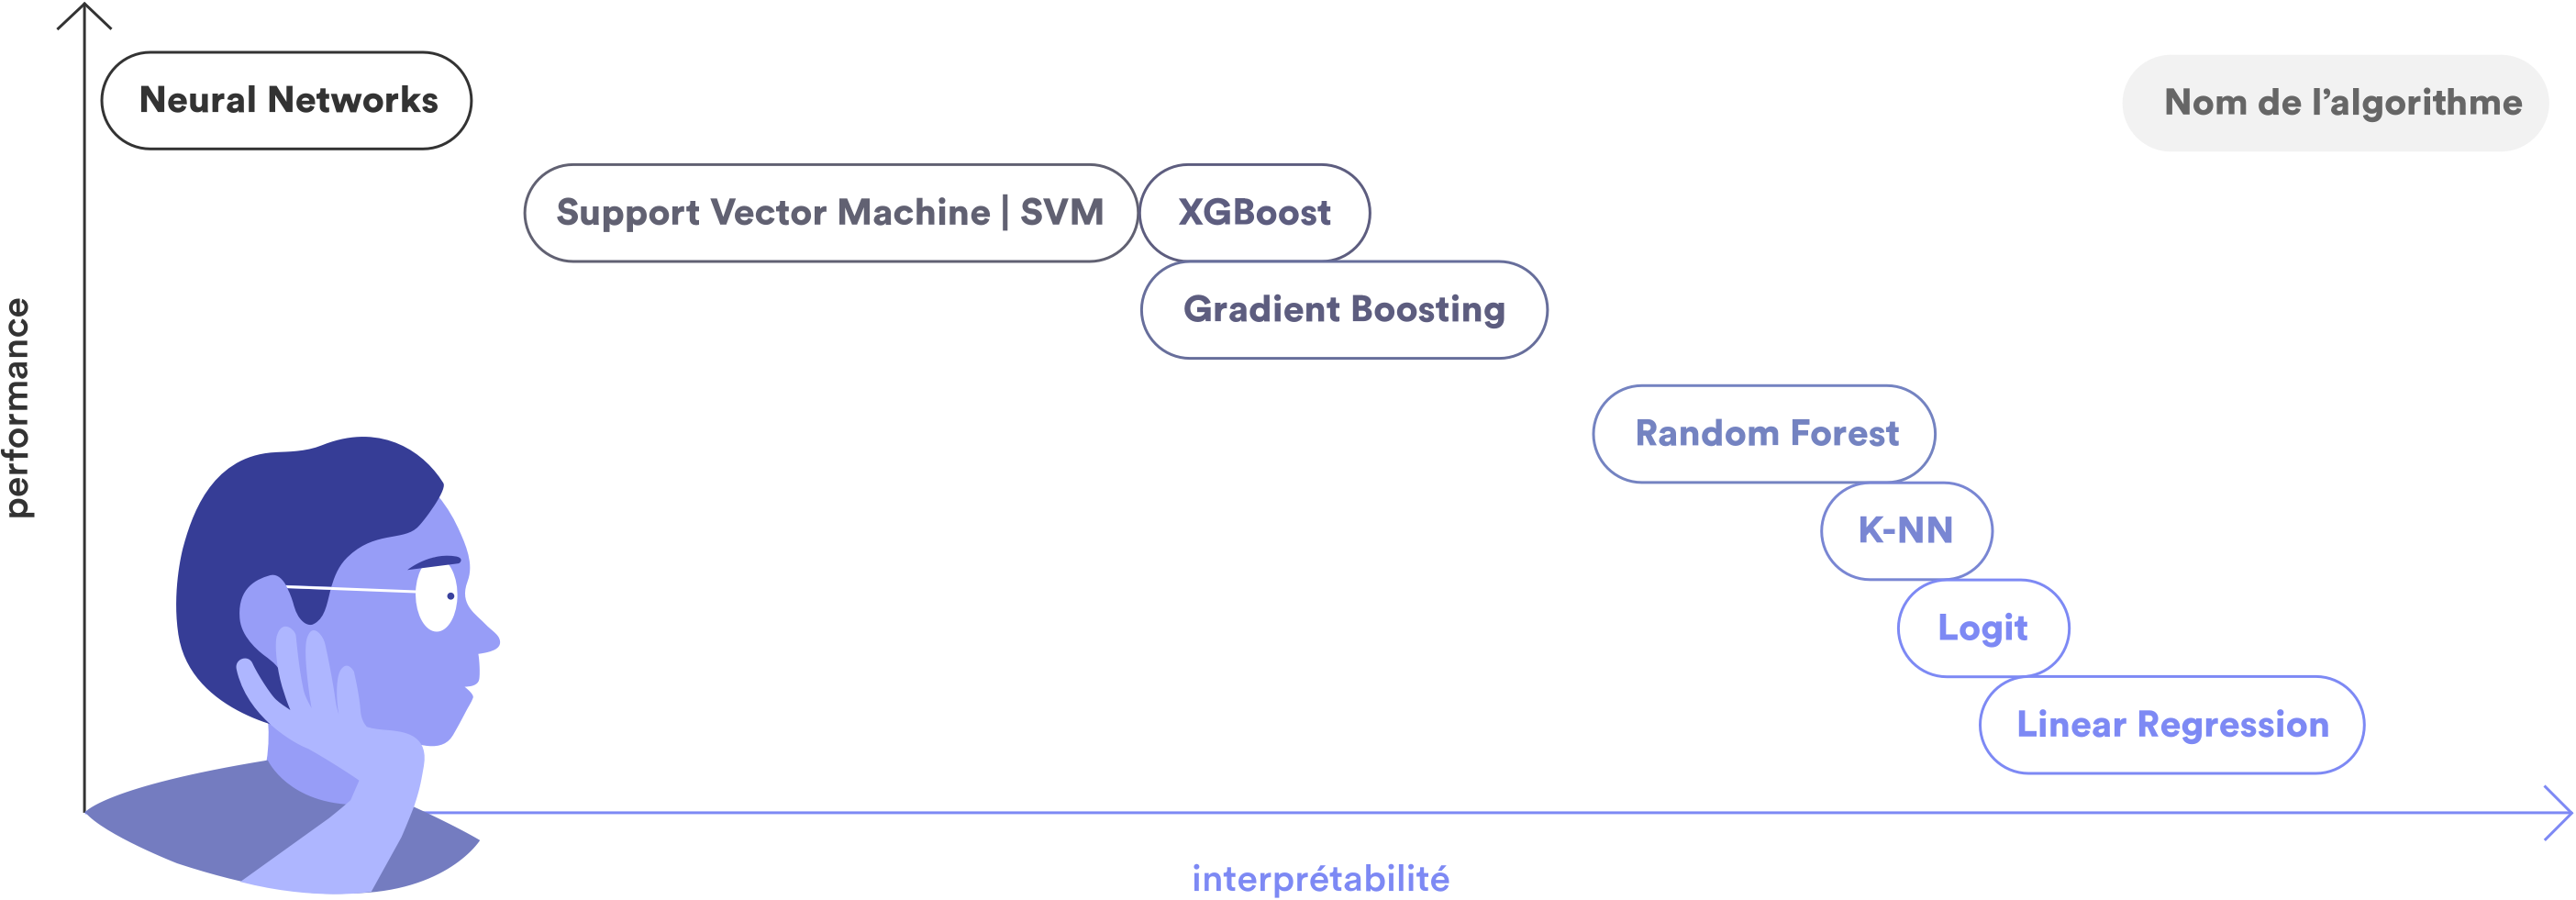
\includegraphics[width=\textwidth]{images/interpretabilite_ia.png}
    \caption{Interprétabilité d'un algorithme \citep{data_for_good_serment_2018}}
    \label{fig:interpretabilite_ia}
\end{figure}

\paragraph{}
Alors, la résignation d’avoir des algorithmes compréhensibles par l’humain est-elle nécessaire ? Non, rentre en jeu la notion d’explicabilité d’un modèle. Ce terme renvoie principalement à la question "Pourquoi ?", la capacité à répondre à ce questionnement lors d’une décision ou prédiction d’un modèle \citep{gilpin_explaining_2018}.

\paragraph{}
Concernant cette nouvelle problématique, l’explicabilité est plus facile à concevoir, pour reprendre la notion de boîte noire, il suffit de modifier les données en entrée pour voir comment cela influe sur le résultat obtenu par l’algorithme.

\paragraph{}
La transparence d’une intelligence artificielle passe également par la publication du code composant cette dernière publiquement, c’est-à-dire un code open-source\footnote{L’open source est une philosophie de développement désignant le fait d’ouvrir le code à tous, librement.}. Cela est bien problématique quand il s’agit d’algorithmes réalisés en entreprise et ne voulant pas publier leur réalisation au grand public.

\paragraph{}
Les explications à une non-<publication peuvent être diverses. Les plateformes comme Youtube ou Google ne publieront pas leur algorithme par nécessité d’éviter les abus afin de tirer profit d’une potentielle faille. OpenAI, eux bien qu’ils prônent cette idéologie de partager le code des IA afin de pouvoir mieux prévenir l’éthique des futures intelligences artificielles, ont décidé, de publier uniquement une partie de l’IA GPT-2 \citep{radford_language_2019}, IA capable d’écrire des textes catégorisables de "fake news"\footnote{Traduction : Informations fausses. Il s’agit de nouvelles pouvant sembler vraies dans la forme, mais fausses dans le fond.} et difficilement discernables par l’humain. La justification correspond au choix d’éprouver davantage le modèle et de laisser le temps de préparer des solutions aux problématiques amenées par ce modèle.

\paragraph{}
Cette difficulté, de rendre toutes les IA transparentes et compréhensibles par tous reflète bien le fossé séparant une éthique parfaite aujourd’hui et l’idéalisation qu’il est possible de faire, d’autant plus quand les algorithmes intelligents affectent notre quotidien. La responsabilité d’identifier les biais et comment rendre l’IA transparente revient dans un premier temps aux personnes s’occupant de la création des intelligences artificielles.

\subsubsection{Les créateurs des IA, architectes de notre quotidien}

\paragraph{}
Ces dernières années, le quotidien d’une grande majorité de Français (ou autres habitants d’un pays catégorisé comme occidental) a énormément changé. En effet, suivant un rythme de croisière, les algorithmes dictant le style de vie du quotidien se sont retrouvés omniprésents : Facebook, Google, Netflix, Youtube et d’autres. Ces intelligences artificielles affectent-elles notre vision du monde, notre vie au quotidien ? Les data scientists\footnote{Développeur.euse en charge de créer le modèle qui composera l’intelligence artificielle.}, parents des IA peuvent bien changer notre quotidien au travers de leurs enfants.

\paragraph{}
Facebook, le réseau social ayant le plus d’utilisateurs dans le monde avec deux milliards 320 millions d’utilisateurs \citep{clement_global_2019}, a déjà eu l’occasion de prouver son influence sur l’humeur des utilisateurs. L’algorithme, qui choisit quelles publications un utilisateur pourra voir sur son fil d’actualité, possède une puissance d’impact sur nos émotions : si l’IA affiche une majorité de publications uniquement positives ou uniquement négatives sur une semaine, les publications, et donc l’humeur, des utilisateurs suivra l’état d’esprit auquel ils ont été exposés \citep{kramer_correction_2014}. Une telle constatation pose alors la question de l’influence que peut avoir l’idéologie des concepteurs de l’algorithme qu’ils en aient conscience ou non.

\paragraph{}
Sur Internet, il est possible de nos jours de trouver des réponses à nos questions sur des moteurs de recherche comme Google, leader de ce domaine. Il est surprenant de savoir que depuis 2017, plus de vidéos Youtube sont vues que de recherches Google sont effectuées \citep{desjardins_infographic:_2018}. La promotion de vidéos par l’algorithme de Youtube, fait rentrer ses utilisateurs dans des bulles correspondant à "leurs goûts". Au même détriment que Facebook, la vision du monde d’un internaute est alors biaisée par cette plateforme.

\paragraph{}
Cette source de média en ligne, étant alors une source irréfutable de distraction, connaissance ou encore de culture, est pour chaque utilisateur une urne remplie de vidéos catégorisées. Le risque dans un environnement de ce type est qu’il y ai une fixation sur une catégorie précise de vidéos (poussant alors le biais de confirmation s’il s’agit d’une idéologie). Mickaël Launay soutient, qu’en mathématiques, un tel milieu ségrègue les utilisateurs en deux ensembles : les conformistes et anti-conformistes \citep{launay_urnes_2012}. Les conformistes auront uniquement des vidéos qui leur correspondent, mais pour la seconde catégorie les vidéos seront d’un certain pourcentage correspondant à leur goût et le reste étant dans la catégorie conforme.

\paragraph{}
L’influence des intelligences artificielles sur nos humeurs et opinions dans notre utilisation d’internet quotidienne est irréfutable. Bien que l’objectif de ses algorithmes est de maintenir ses utilisateurs le plus longtemps sur la plateforme, ces IA peuvent, malgré elles, pousser une addiction idéologique chez les utilisateurs. Les data scientists possèdent-ils les appétences pour des réflexions aussi poussées que les impacts sociaux issus de leurs intelligences artificielles ?

\paragraph{}
Une majorité de data scientists sont issus de formation statistique, mathématiques ou encore informatique. Cela contraint déjà sur la notion de connaissance du domaine sur lequel une IA sera développée. La responsabilité de ceux qui produisent les algorithmes intelligents est de mentionner dans leurs discours les limites de leurs travaux, mais aussi de fournir un maximum d’informations aux personnes prenant les décisions et législateurs qui devront évaluer l’impact potentiel de ces apports sur la société \citep{cointe_ethical_2017}. Si cette responsabilité n’est pas respectée ou pire, que les limites sont omises volontairement afin de profiter à l’entreprise créatrice alors les répercussions peuvent être de l’ordre des biais impactant des femmes et hommes n’en ayant point conscience.

\paragraph{}
L’objectif d’une conscience de l’éthique pour que les intelligences artificielles soient plus transparentes et moins biaisées, qu’elles soient plus justes, est bien présent dans la communauté des chercheurs. Malheureusement la conscience de cette problématique n’est pas majoritaire et dans le but de sensibiliser sur ce sujet, l’association Data for Good a mis en place le "Serment d’Hippocrate pour Data Scientist" \citep{data_for_good_serment_2018} prenant en compte ces problématiques. Bien que cela ne soit encore qu’un engagement n’ayant pas de valeur juridique, peut-être cela évoluera dans les années qui suivent.

\paragraph{}
Les valeurs qui sont évoquées dans ce document peuvent se résumer au nombre de cinq. Dans un premier temps, l’intégrité scientifique et la rigueur, puis la transparence vis-à-vis de l’information compréhensible par le plus de parties prenantes possibles. L’équité suit, afin de veiller à une égalité et d’éviter la discrimination de groupes. L’avant-dernière concerne le respect de la vie privée des personnes qui peuvent être touchées par les travaux réalisés et enfin la responsabilité poussant à assumer tout manquement ou en cas de conflit d’intérêt.

\paragraph{}
Cette conscience ne doit pas se limiter qu’aux concepteurs des IA, il est nécessaire que cela soit multi-disciplinaire. Chaque acteur intervenant lors de la création d'un algorithme intelligent doit agir pour tendre vers une intelligence artificielle de confiance.

\subsection{Une IA de confiance selon la Commission Européenne}
\label{subsec:ia_confiance_com_ue}

\paragraph{}
Le domaine de recherche sur l'intelligence artificielle et l'éthique est assez récent et nous pouvons même recenser jusqu'à plus 70 documents ont été publiés entre 2016 et 2019 \citep{algorithm_watch_ai_2020}. Les différents auteurs sont principalement des gouvernements, des académies et des entreprises \citep{morley_what_2019}. Le but des auteurs de ces documents est qu'en définissant des principes théoriquement, de façon abstraite, ces principes permettront d'agir comme contraintes normatives \citep{turilli_ethical_2007} sur ce qui doit être fait et ce qui ne doit pas être empêché pour l'utilisation d'un algorithme. En d'autres termes, il s'agit de principes qui permettront de garantir une IA éthique.

\paragraph{}
Parmi les documents publiés, nous allons nous intéresser à celui qui a été écrit par un groupe expert indépendant sur le sujet de l'IA et qui nous concerne directement car il a été rédigé par la Commission Européenne : ``Lignes directrices en matière d'éthique pour une IA de confiance'' \citep{commission_europeenne_ethics_2019}. En prémisse du document, il est stipulé que pour obtenir une intelligence artificielle de confiance il est nécessaire de respecté trois caractéristiques : 

\begin{itemize}
  \item Licité : respect de législations et réglementations applicables.\footnote{Le document de la Commission Européenne ne traite pas l'aspect licite.}
  \item \uppercase{é}thique : assure l'adhésion de valeurs et de principes éthiques.
  \item Robuste : garantie sur le plan technique et social d'éviter de causer des préjudices involontaires.
\end{itemize}

\paragraph{}
Basé sur ces fondements caractérisants une IA de confiance, sept exigences dites ``essentielles'' sont décrites qui permettent de diriger vers un idéal. Les concepts détaillés reste théoriques. Ces différentes exigences sont présentées dans la Figure \ref{fig:7_exigences}.

\begin{figure}[hbt!]
  \centering
  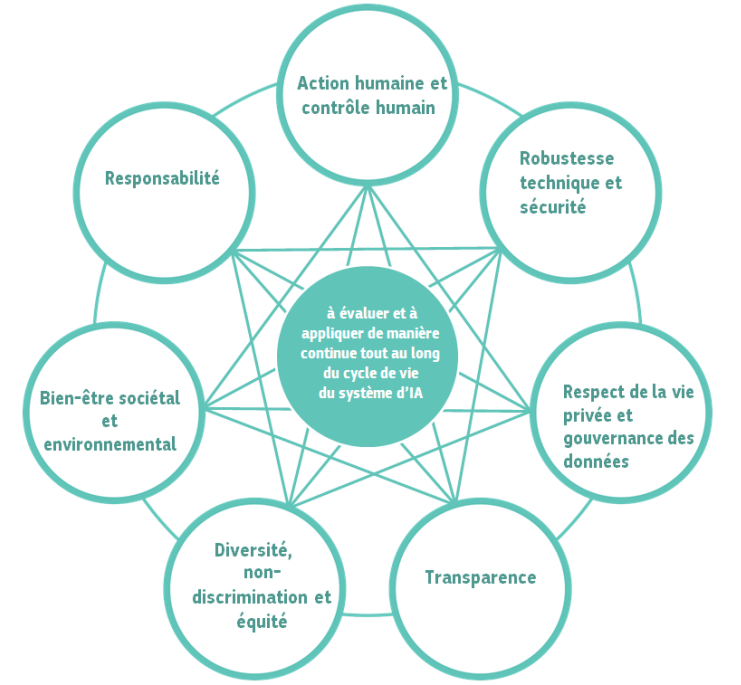
\includegraphics[width=0.7\textwidth]{images/7_exigences_commission.png}
  \caption{interrelation des sept exigences: elles revêtent toutes une importance égale, elles se soutiennent mutuellement et devraient être appliquées et évaluées tout au long du cycle de vie d’un système d’IA. \citep{commission_europeenne_ethics_2019}}
  \label{fig:7_exigences}
\end{figure}

\paragraph{1. Action humaine et contrôle humain} Les systèmes d'algorithmes intelligents se doivent d'être centré autour des humains : ils doivent respecter l'autonomie humaine en respectant les Droits Fondamentaux voire ces systèmes, s'ils le peuvent, devrait les renforcer. Les femmes et hommes doivent garder l'action sur l'IA en prenant par exemple des décisions à partir de l'algorithme tout en pouvant protester face à la décision d'une machine. Enfin le contrôle humain est essentiel par l'approche ``human-in-the-loop'', ``human-on-the-loop'' ou ``human-in-command'' qui signifient respectivement : l'humain qui intervient dans le processus, qui supervise le processus et qui reste aux commandes. 

\paragraph{2. Robustesse technique et sécurité} Cette exigence est liée au principe de prévention de toute atteinte. Pour assurer une robustesse technique il faut garantir un système d'information sécurisé et résilient. De plus, une IA peut être soumises à des attaques comme par exemple la modification des données en entrée pour avoir un meilleur résultat. Ces attaques doivent être anticipées pour être évitées. La Commission ajoute que la mise en place de plans de secours et la sécurité générale de l'environnement dans lequel évolue l'algorithme sont à assurer. Enfin, un modèle qui est déployé doit être valider par des mesures de précision et les données sur lesquelles il s'est entraînées doivent être fiables.

\paragraph{3. Respect de la vie privée et gouvernance des données} Il s'agit là d'un droit fondamental et le Règlement Général de la Protection des Données (règlement numéro 2016/679) rentre dans ce cadre en stipulant que les données d'un clients doivent être protégées. De plus, si l'algorithme assimile une grande quantité de données pour faire ses prédictions, il y a un risque qu'il arrive à déduire de lui même des données personnelles (voire sensibles) comme l'âge, l'orientation sexuelle, le sexe ou encore les opinions politiques d'une personne. Dans la continuité, les données doivent être de qualité et leur intégrité doit être préservée. 

\paragraph{4. Transparence} Cette exigence est liée au principe de l'explicabilité (voir section \ref{subsec:explicabilite}), c'est à dire à pouvoir comprendre le modèle qui a été fabriqué. Pour assurer cela, le cycle de vie de la donnée doit être traçé et documenté. Un modèle a besoin de respecter l'explicabilité : c'est-à-dire qu'il doit être possible de fournir une explication en langage naturel. De plus, si pour une problématique donnée il est possible de choisir un type d'algorithme considéré comme plus interprétable et qui obtient des performances similaires, alors il est préconisé de le choisir. Pour fini, la communication n'est pas à négliger pour que les utilisateurs comprennent de ce qu'il en retourne concernant le modèle. 

\paragraph{5. Diversité, non-discrimination et équité} Le respect du principe d'équité est essentiel pour permettre d'avoir une IA de confiance. Un algorithme se doit d'être accessible avec une conception universelle peut importe l'âge, le sexe, les capacités ou les caractéristiques d'un humain. Comme discuté dans la section \ref{subsec:biais}, l'absence de biais injuste est un critère fondamental dans le cas où l'algorithme peut avoir un préjudice pour un individu (comme l'obtention d'un crédit ou le recrutement dans une entreprise). \uppercase{à} titre préventif, il est souhaitable de faire participer les parties prenantes concernées par l'IA en question.

\paragraph{6. Bien-être sociétal et environnemental} Cette exigence est liée à la précédente puisque l'omniprésence des algorithmes sur nos réseaux sociaux et dans notre quotidien ne devraient pas avoir d'incidences sociales sur nos relations et liens sociaux. \uppercase{é}galement, l'aspect environnemental avec la quantité de données utilisées et le temps d'entraînement d'un modèle, est à ne pas négliger car pour certains modèles la consommation énergitique peut être très importantes.

\paragraph{7. Responsabilité} Lorsqu'une IA est mise à disposition en publique ou bien mise en production, il faut anticiper les problèmes potentiels avec la possibilité d'auditer l'algorithme, ce qui oblige à bien documenter. En cas d'incidences négatives, il convient de garantir la capacité de les minimiser et de les documenter pour éviter des problèmes similaires dans le futur. Enfin si une incidence négative à lieu pour une personne donnée, il convient de préparer des mécanismes pouvant permettre de faire recours sur la décision.

\paragraph{}
Ces exigences bien que non exhaustifs, ils ont le bénéfice de couvrir une grande partie de la théorie sur ce que devrait être une IA éthique et de confiance. La Commission propose en plus des exemples de méthode pour assurer une IA de confiance en cohésion avec les exigences décrites précédemment. Ces méthodes sont découpées en deux catégories : méthodes techniques et non techniques (pages 26 à 29).

\paragraph{Méthodes techniques :} Architectures pour une IA digne de confiance , Éthique et état de droit dès la conception (X dès la conception), Méthodes d’explication, Essais et validations et Qualité des indicateurs de service.

\paragraph{Méthodes non techniques :} Réglementation, Codes de conduite, Normalisation, Certification, La responsabilité au moyen de cadres de gouvernance, Éducation et sensibilisation pour encourager un état d’esprit éthique, Participation des parties prenantes et dialogue social et Diversité et équipes de conception inclusives.

\paragraph{}
En conclusion, la Commission reconnait ``les effets positifs que les systèmes d’IA ont déjà et continuerons à avoir, tant d’un point de vue commercial que pour la société.'' Mais insiste sur l'importance de mettre au point des IA dignes de confiance, d'autant plus dans un contexte où les machines sont omniprésentes et prennent des décisions pouvant impacter notre vie profondémment.

\subsection{Les Dilemmes Moraux pour les Machines}

\paragraph{}
L’émergence des intelligences artificielles et la possibilité du passage de la singularité fait apparaître la difficulté à aligner la morale de l’homme à celle de la machine : c’est le problème de l’alignement, comment une machine devant un dilemme moral devrait raisonner et agir.

\subsubsection{Expliciter la morale des humains : Moral Machine}

\paragraph{}
Le futur qui admet une intelligence artificielle ayant un intellect supérieur à l’homme plonge dans les débats éthiques et culturels, le problème de l’alignement oblige l'écriture noir sur blanc de "la morale" souhaitée pour une machine. Cette démarche est nécessaire, la morale qu’une machine aurait dans le futur est difficilement conceptualisable pour les humains.

\paragraph{}
Pour ce faire, il serait intéressant d’avoir une liste de règles bien définies comme les célèbres trois lois de la robotique d’Isaac Asimov. Bien qu'elles soient recentrées sur l’atteinte et l’obéissance à l’être humain, le raisonnement est à pousser au maximum.

\paragraph{}
Une expérience de pensée assez célèbre pour illustrer cette nécessité serait le cas d'une voiture autonome, dans un contexte où les freins ne fonctionneraient pas en face de piétons, qui la voiture devrait choisir de tuer. Le MIT a proposé une étude nommée "Moral Machine", offrant des choix en fonction de l’âge, du nombre, du sexe, de la classe sociale (un exemple sur la figure \ref{fig:moral_machine}). Les résultats montrent une divergence entre les cultures. En effet pour la question de l’âge, la jeunesse sera préférée pour des pays dit occidentaux à contrario des pays asiatiques favorisant les personnes âgées \citep{awad_moral_2018}.

\begin{figure}[hbt!]
    \centering
    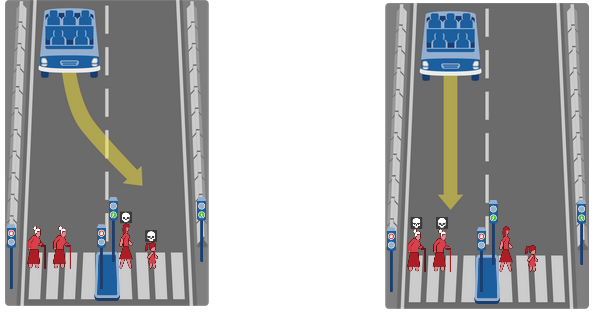
\includegraphics[width=\textwidth]{images/moral_machine.png}
    \caption{Expérience "Moral Machine" du MIT, ici le choix se pose entre deux femmes agées ou une petite fille accompagné d'une femme.}
    \label{fig:moral_machine}
\end{figure}

\paragraph{}
C’est déjà une étape importante puisque la réflexion émerge sur des questions qui sont d’actualité, e.g. la Californie autorisant les voitures autonomes à circuler sans conducteur \citep{shepardson_waymo_2018}, et permettent de commencer une réflexion plus profonde sur l’avenir de l’IA et d’une morale peut être relative à un pays. Tout ceci n’est que spéculation, les lois ne sont pas encore adaptées, les éthiques divergent énormément selon les pays.

\paragraph{}
Alors, si les lois sont plus difficilement malléables que les mœurs en rapport aux machines, des travaux ont été réalisés pour permettre dès l’apprentissage de l’algorithme intelligent de pouvoir aligner la morale humaine à celle de la machine.

\paragraph{}
Une solution pourrait être de découper la fabrication d’une IA en cinq parties : la collecte de données fiables, le modèle d’apprentissage basé sur la représentation du monde (issu des données collectées), la compréhension du modèle ainsi que le choix de la mesure de performance du modèle, définir les incentives\footnote{Il s’agit de source de motivation pour réaliser une action, e.g. une médaille lors d’une compétition sportive.} en jeux et enfin le renforcement de l’apprentissage dans le temps \citep{hoang_roadmap_2018}. Cette méthodologie s’axe sur tout le développement d’une IA, le point de départ pour parvenir à réaliser cela est de pouvoir conceptualiser les valeurs humaines.

\paragraph{}
La collecte des valeurs humaines dans le but de l’alignement passera par des questionnaires pour les humains, le problème étant que les réponses qui seront fournies posséderont des défauts : les biais, le manque de connaissances dans le domaine, les capacités cognitives limitées ou encore la culture dans laquelle évolue la femme ou l’homme. La nécessité d’inclure des sociologues avec chercheurs en IA est importante afin de répondre à la question de savoir si les humains donneront une bonne réponse à la question \citep{irving_ai_2019}.

\paragraph{}
La forme de l’apprentissage de la morale peut être appliquée sous diverses formes, par exemple l’une pourrait être par observation du comportement des autres et en ajustant la morale par l’observation des conséquences \citep{cointe_ethical_2017}. Une autre viserait plus l’apprentissage par le débat, poussant alors la justification des intelligences artificielles dans leurs recoins \citep{irving_ai_2019}.

\paragraph{}
La sensibilisation sur la problématique d’une morale pour les IA ainsi que le problème de l’alignement est primordiale. Il est important de travailler sur ces problèmes sur le plan technique en formant les actuels et futurs data scientists sur la question éthique et en rajoutant des sociologues pour aider sur les réponses aux questions de l’ordre moral, en d’autres termes, l’éducation et le social seront deux secteurs clés des avancées dans la transparence des algorithmes intelligents.

\paragraph{}
Tous ses problèmes que soulèvent les algorithmes intelligents, bien heureusement, suscitent un intérêt pour la communauté de chercheurs ainsi que pour les instances gouvernementales. Une volonté commune est née avec pour objectif de théoriser ce que peut être une intelligence artificielle éthique.

\subsubsection{La décision par l'Aléatoire : Alexei Grinbaum}

\begin{quotation}
  ``Les choix éthiques ne doivent être fait que par les Hommes.''
\end{quotation}
\rightline{{\rm --- \citep{grinbaum_conversation_2019}}} 

\paragraph{}
Dans son livre ``Les robots et le Mal'' \citep{grinbaum_les_2019}, Alexei Grinbaum, philosophe et physicien, propose une méthode de résolution de conflits moraux lorsqu'une machine se doit de faire un choix moral : faire ce choix en le tirant au sort.

\paragraph{}
Dans les premières pages de son livre, il évoque la première de couverture du journal ``The Economist'' du 19 décembre 2009 qui représente Adam et Eve du mythe tenant un appareil Apple (voir Figure \ref{fig:the_economist}). Ce couple correspond à la métaphore du bien et du mal, de la condition humaine, cette couverture a pour sens le fait de soulever la question de comment la machine modifie la condition humaine. Il en va de soit que nous pouvons le pousser jusqu'à l'intelligence artificielle.

\begin{figure}[hbt!]
  \centering
  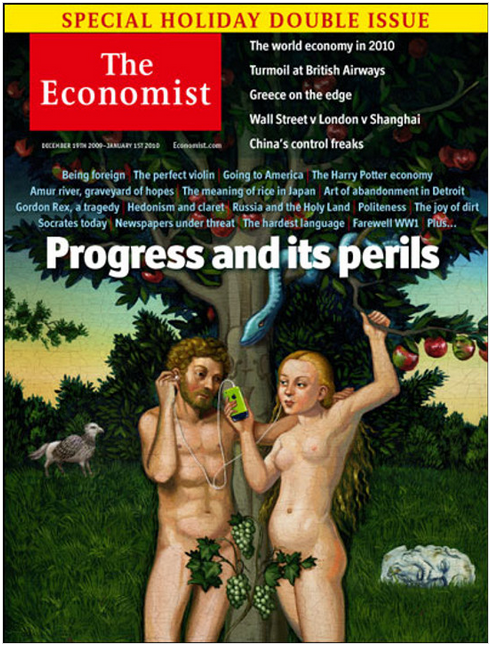
\includegraphics[width=0.4\textwidth]{images/the_economist_200091219.png}
  \caption{Première de couverture de l'édition du 19 décembre 2009 de ``The Economist'' \cite{theeconomist_progress_2009}.}
  \label{fig:the_economist}
\end{figure}

\paragraph{}
Si nous revenons sur les résultats de l'étude étudiée dans la section précédente, nous avons constaté que le comportement d'une voiture autonome devrait varié en fonction des cultures et des moeurs. Cela semble cohérent, mais est-ce que la morale d'une voiture autonome doit être faite par pays, par catégorie sociale ? De plus, est-ce qu'une voiture autonome sur Paris avec un français à l'intérieur devrait-elle se comporter différement qu'avec un passager brésilien ou australien ?   

\paragraph{}
Ces questions poussent à définir exactement une morale en fonction, mais cela relève de l'impossible car le nombre de possibilité de conflits moraux est immenses. De plus, que devrait prendre en compte la fonction qui ferait le choix de favoriser une personne plutôt qu'une autre ? Son cercle d'ami, sa famille, son apparence ou ses goûts musicaux ? La complexité d'une telle fonction peut également remettre en cause la responsabilité d'une machine sur le plan légal.

\paragraph{}
Alexei Grinbaum affirme qu'il ne pense pas ``qu’une machine puisse être considérée comme une personne juridique puisque ce n’est pas une personne'' \citep{grinbaum__2019}, en effet il propose de plutôt partager la reponsabilité entre les agents humains qui interviennent lors de la création de l'algorithme : les programmateurs, la société qui produit l'IA, l'utilisateur qui influe sur la décision de l'algorithme ou encore sur les personnes sélectionnant les données qui serviront à entraîner le modèle.

\paragraph{}
Alors l'une des solutions envisageables serait de prendre une décision basée sur un tirage au sort. Bien que les humains n'aiment pas vivre dans l'incertitude, l'aléatoire permet de résoudre les conflits moraux sans préjugé ni préjudice. Prenons le cas du dilemme pour lequel une voiture autonome pourrait avoir : qui sauvé le cas échéant. Un tirage au sort permettra de ne pas remttre en cause la malveillance de la machine, même si les conséquences peuvent en être dramatiques.

\paragraph{}
A. Grinbaum rappelle qu'une situation de conflit moral reste assez rare et que par conséquent l'impact dans une société de l'application par le hasard restera minime globalement. De plus, la difficulté deviendrait de créer un système capable detecter un conflit moral pour pouvoir le résoudre de façon aléatoire. Nous pouvons dire que le calcul moral qui est à priori très complexe se réduit à un jet de dés.

\section{Synthèse}

\paragraph{}
Pour rappel, la problématique de ce mémoire pose le cadre sur deux domaines : l’intelligence artificielle et l’éthique. Dans ce chapitre, dans un premier temps, l’histoire de l’intelligence a été évoquée avec notamment le test de Turing (voir section \ref{sec:ia}). Celui-ci pouvant symboliser une première étape pour atteindre le passage de la singularité, qui, selon les experts du domaine aurait plus de cinquante pourcents de chances d’être atteinte d’ici cinquante ans (voir Figure \ref{fig:chrono_estim_ia}).

\paragraph{}
Dans un second temps, une introduction à la morale, avec entre autres son origine historiquo-philosophique vu par Nietzsche (voir section \ref{subsec:ethique_origine_bon}). Différentes morales ont été évoquées d’un point de vue philosophique démontrant une complexité déjà humaine à trouver une morale pouvant plaire au plus grand nombre (voir section \ref{subsec:ethique_jugement_chacun}). Enfin, nous avons vu la vision de la morale dans la Science, notamment avec l'approche du culturalisme et celle du naturalisme \ref{subsec:morale_science}.

\paragraph{}
C’est pour cela qu’en dernier lieu, la section \ref{sec:ia_ethique} rentre dans les problèmes soulevés par l’intelligence artificielle sur le plan de l’éthique et présente un premier état de l’art sur les études existantes. Différents aspects ont été cités : les biais, la transparence des algorithmes, l’influence actuelle des IA avec les data scientists et enfin une vision qui pourrait permettre d’expliciter la morale des intelligences artificielles. Sans oublier la théorie de ce que devrait être une IA éthique au travers des écrits de la Commission Européenne.

\paragraph{}
La problématique peut alors se découper sur deux points de l’éthique : une IA socialement responsable et la supervisation de son éthique.

\paragraph{}
Déterminer si une intelligence artificielle est socialement responsable revient à déterminer les impacts sociaux de cette dernière, qui s’inscriront dans la démarche de poser les questions des conséquences que celui-ci peut avoir pour un groupe d’individus ou pour un cas particulier, qui est concerné et dans quels buts.

\paragraph{}
La supervisation de l'éthique d'une IA a pour différence d'être plus technique, décliner tous les aspects des critères décrits par la Commission Européenne afin de répondre à la question : ``Est-ce cette intelligence artificielle est éthique ?''

\paragraph{}
La vision qui ressort est celle d’une "méta-IA" soit d’une boîte à outil, d’un guide qui pourrait s’adapter aux différentes intelligences artificielles. Dans le chapitre suivant, je présente les solutions existantes et comment les regrouper dans un outil pouvant garantir une IA de confiance.

% ======= SOLUTION ===== %
\newpage
\chapter{Solution : une boîte à outils transparente}

\paragraph{}
Dans la partie précédente, nous avons évoqué les travaux théoriques concernant la notion d'intelligence artificielle éthique (ou de confiance selon la Commission Européenne). La Commission n'est pas la seule organisation qui a publié des principes pour garantir l'éthique dans un système intelligent (CF section \ref{subsec:ia_confiance_com_ue}).

\paragraph{}
\begin{quotation}
  ``La disponibilité de ces principes ``convenus" encourage mais n'entraîne pas encore de changement réel dans la conception des systèmes algorithmiques. Comme on peut le constater, la quasi-totalité des lignes directrices produites à ce jour laissent penser que des solutions techniques existent, mais très peu d'entre elles fournissent des explications techniques. En conséquence, les développeurs sont frustrés par le peu d'aide offerte par des principes très abstraits lorsqu'il s'agit de ``travail de jour".''
\end{quotation}
\rightline{{\rm --- \citep{morley_what_2019}}} 

\paragraph{}
Nous sommes donc dans une impasse pour les développeurs d'IA : des entreprises et des gouvernements expliquent ce que doit être une IA éthique, mais s'abstiennent sur les solutions techniques. Une partie des publications sur le sujet fournissent des questionnaires plus ou moins complexes pour faire respecter les principes, ce qui reste loin de la réalité d'un concepteur d'IA.

\paragraph{}
Dans cette section, nous allons découvrir des outils et des méthodes mathématiques qui répondent techniquement aux questions soulevés par la Commission Européenne. De plus, ces outils n'étant pas centralisé au même endroit, il est nécessaire de les regrouper dans un même outil qui par conséquent est une boîte à outil : TransparentAI. 

\section{Travaux connexes}

\paragraph{}
Cette section a pour but d’analyser des travaux portant sur la réflexion éthique au sein du domaine de l’intelligence artificielle. Les travaux qui seront présentés proviennent de réflexions mathématiques. L’introduction de ces différentes approches est importante puisque certaines sont liées à des outils techniques qui seront réutilisés dans ce mémoire, notamment avec la création d’un outil technique.

\subsection{Analyser les biais au sein d'une IA}

\paragraph{}
Nous avons vu dans la section \ref{subsec:biais} que les biais au sein d'un algorithme peuvent avoir des conséquences importante pour un être humain. Il est fondamental de pouvoir identifié ces biais et de les atténuer si nécessaire. 

\subsubsection{Mesure des biais : calculer l'impact social}

\paragraph{}
La mesure de biais dans un algorithme n'est pas absolu : il existe différentes méthodes pour pouvoir les mesurer, chacune possède sa spécificité. Nous allons voir quatre méthodes qui permettent de couvrir un potentiel impact social de l'algorithme.

\paragraph{}
Dans les définitions qui suivent, nous allons utiliser les termes mathématiques suivants :

\begin{itemize}
  \item $\hat{Y}$ : c'est la sortie d'un modèle, la prédiction
  \item $D = privileged$ : il s'agit de la partie des données pour laquelle nous considérons que la personne est privilégiée sur un attribut social (e.g. genre de la personne).
  \item $D = unprivileged$ : il s'agit de la partie des données pour laquelle nous considérons que la personne n'est pas privilégiée sur un attribut social (e.g. genre de la personne).
\end{itemize}

\paragraph{}
Par exemple, prenons une IA cherchant à prédire si une personne est en capacité de rembourser un crédit immobilier : $\hat{Y}$ sera la probabilité qu'il y parvienne, pour l'attribut social du genre de la personne, $D = privileged$ sera les hommes et $D = unprivileged$ les femmes.

\paragraph{}
Pour ces mesures de biais, le modèle est une classification binaire, il ne peut retourner que 1 (resultat dit positif) ou 0 (résultat dit négatif). De plus, nous pouvons les associer avec les valeurs réelles pour évaluer l'efficacité du modèle ; est-ce que la prédiction du modèle est vraie ou fausse ?

\begin{center}
  \begin{tabular}{ |c|c|c|c| } 
   \hline
   Prédiction $\hat{Y}$ & Réalité $Y$ & Terme associé & Traduction \\ 
   \hline
   0 & 0 & TN (True Negative) & Vrai Négatif \\ 
   1 & 0 & FP (False Positive) & Faux Positif \\ 
   0 & 1 & FN (False Negative) & Faux Négatif \\ 
   1 & 1 & TP (True Positive) & Vrai Positif \\ 
   \hline
  \end{tabular}
\end{center}

\paragraph{}
Grâce à ces indicateurs, il est possible d'obtenir des mesures de performance du modèle comme la Justesse (CF équation \ref{eq:accuracy}). Nous allons en voir deux qui seront utilisées dans deux des mesures de biais : le ``True Positive Rate'' ($TPR$) où ``Taux de Vrai Positif'' et le ``False Positive Rate'' ($FPR$) où ``Taux de Faux Positif''.

\begin{equation}\label{eq:tpr}
  \text{True Positive Rate (TPR)} = \frac{TP}{TP + FN}
\end{equation}
\begin{equation}\label{eq:tpr}
  \text{False Positive Rate (FPR)} = \frac{FP}{FP + FN}
\end{equation}

\paragraph{Statistical Parity Difference}
\begin{equation}\label{eq:stat_par_diff}
  Pr(\hat{Y} = 1 | D = unprivileged) - Pr(\hat{Y} = 1 | D = privileged)
\end{equation}

\paragraph{}
Calcule la différence du taux de résultats favorables reçus par le groupe non privilégié par rapport au groupe privilégié. La valeur idéale de cette mesure est 0. Une valeur inférieure à 0 implique un bénéfice plus élevé pour le groupe privilégié et une valeur supérieure 0 implique un bénéfice plus élevé pour le groupe non privilégié.

\paragraph{}
Par exemple, avec le modèle du crédit immobilier sur l'attribut du genre, un résultat de -0,07 implique que les hommes sont prédit comme capable de rembourser leur prêt 7\% plus souvent que les femmes.

\paragraph{Equal Opportunity Difference}

\begin{equation}\label{eq:eq_oppo_diff}
  TPR_{D = unprivileged} - TPR_{D = privileged}
\end{equation}

\paragraph{}
Cette mesure est calculée comme la différence des taux réellement positifs entre les groupes non privilégiés et les groupes privilégiés. Le taux de vrais positifs est le rapport entre les vrais positifs et le nombre total de vrais positifs pour un groupe donné. La valeur idéale est 0, une valeur inférieure à 0 implique un bénéfice plus élevé pour le groupe privilégié et une valeur supérieure à 0 implique un bénéfice plus élevé pour le groupe non privilégié.

\paragraph{}
Par exemple, avec le modèle du crédit immobilier sur l'attribut du genre, un résultat de -0,04 implique que les hommes, le modèle estime qu'un homme pour rembourser son crédit 4\%  plus souvent que pour une femme.

\paragraph{Average Odds Difference}

\begin{equation}\label{eq:ave_odds_diff}
  1/2 [|FPR_{D = unprivileged} - FPR_{D = privileged}| + |TPR_{D = unprivileged} - TPR_{D = privileged}|]
\end{equation}

\paragraph{}
Calcule la différence moyenne du taux de faux positifs (faux positifs divisé par résultats négatifs) et du taux de vrais positifs (vrais positifs divisé par résultats positifs) entre les groupes non privilégiés et privilégiés. La valeur idéale de cette mesure est 0. Une valeur inférieure à 0 implique un bénéfice plus élevé pour le groupe privilégié et une valeur supérieure à 0 implique un bénéfice plus élevé pour le groupe non privilégié.

\paragraph{}
Par exemple, avec le modèle du crédit immobilier sur l'attribut du genre, un résultat de -0,0215 implique pour un homme, le modèle prédit un résultat correct 2,15\%  plus souvent que pour une femme.

\paragraph{Disparact Impact}

\begin{equation}\label{eq:disp_impact}
  \frac{Pr(\hat{Y} = 1 | D = unprivileged)}{Pr(\hat{Y} = 1 | D = privileged)}
\end{equation}

\paragraph{}
Calcule le rapport entre le taux d'issue favorable pour le groupe non privilégié et celui du groupe privilégié. La valeur idéale de cette mesure est de 1. Une valeur inférieure à 1 implique un bénéfice plus élevé pour le groupe privilégié et une valeur supérieure à 1 implique un bénéfice plus élevé pour le groupe non privilégié.

\paragraph{}
Par exemple, avec le modèle du crédit immobilier sur l'attribut du genre, un résultat de 0,41 implique que les hommes sont prédit comme capable de rembourser leur prêt 2,42 fois plus souvent que les femmes.

\paragraph{Interprétation des mesures} Nous avons donc des mesures qui se complètent pour identifier des biais sur des attributs sociaux. La difficulté n'est pas dans le résultat de mesure de biais, mais dans l'interprétation, il est nécessaire que les humains en charge de l'algorithme arbitre si la mesure est acceptable ou non. Par exemple, si le modèle est biaisé pour le genre (il favorise les hommes par rapport aux femmes), alors la décision de modifier le modèle peut être prise. Mais sur l'attributs de la richesse, la capacité de rembourser un prêt semble lié à cette attribut, par conséquent même si le modèle est biaisé sur la richesse d'un individu, il n'est pas nécessaire de le modifier car pour ce contexte, c'est une observation cohérente.

\subsubsection{AIF360 : AI Fairness 360 par IBM}

\paragraph{}
La discussion autour des biais (voir section \ref{subsec:biais}) poussant à réfléchir comment construire un modèle est une première étape, mais il ne faut jamais exclure la possibilité qu’un ou plusieurs biais s’invitent dans une intelligence artificielle. Pour cela, il est nécessaire de trouver un moyen d’identifier ces biais potentiels ainsi que de parvenir à les limiter.

\paragraph{}
Dans le cadre de cette démarche, l’outil AIF360\footnote{Le nom complet est ``Artificial Intelligence Fairness 360'' qui signifie Intelligence Artificielle Juste 360.} \citep{bellamy_ai_2018} présente divers instruments formant une harmonie pour identifier les biais et les réduire si besoin. Bien que cet outil n’est encore qu’à ses débuts (version 0.3.0, juin 2019), sa qualité n’en est pas moindre. Il se découpe principalement en deux axes : les mesures des biais et les algorithmes de limitation de biais.

\paragraph{}
Les mesures calculeront des biais à partir d’une variable, de préférence correspondant à une segmentation sociale, e.g. sexe d’une personne. Certaines mesures ne s’appuieront que sur le jeu de données et donc identifieront les biais présents dans le jeu de données, d’autres auront besoin des prédictions pour détecter les biais présents dans le modèle. Ces deux groupes permettent d’avoir une vue d’ensemble sur les données et le modèle.

\paragraph{}
Les algorithmes, eux, se catégorisent en trois groupes appelés ``fair-processors''\footnote{Traduction : processeurs justes.} : les ``pre-processors'', ``in-processors'' et ``post-processors''. Les algorithmes de chaque catégorie possèdent globalement les mêmes caractéristiques au détriment du moment de leur utilisation dans la création d’un modèle.

\begin{figure}[hbt!]
  \makebox[\textwidth]{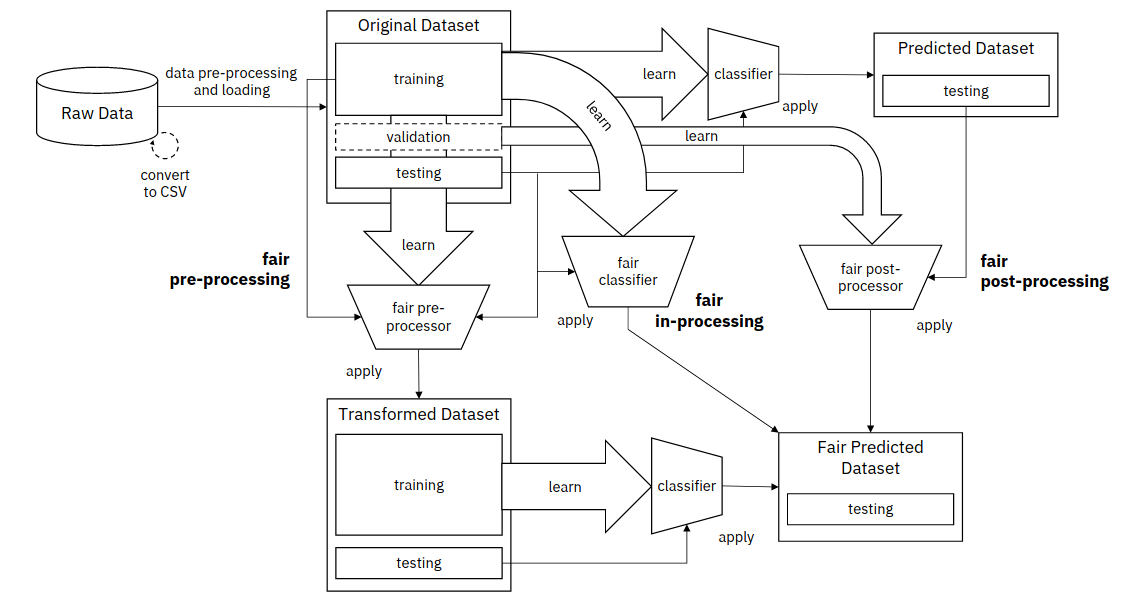
\includegraphics[width=0.9\paperwidth]{images/aif360_pipeline.png}}\caption{``The fairness pipeline", les différents chemins d'utilisation d'AIF360 \cite{bellamy_ai_2018}.}
  \label{fig:aif360_pipeline}
\end{figure}

\paragraph{}
La figure \ref{fig:aif360_pipeline} décrit le pipeline de la création d’un algorithme intelligent, dans un premier temps les données brutes sont transformées en un jeu de données formaté par AIF360. À partir d’ici, pour un ``pre-processor'' la réduction de biais se fait directement avant l’entraînement du modèle, pour un ``in-processor'', le travail s’effectue pendant l’entraînement et enfin pour le ``post-processor'' après l’entraînement.

\paragraph{}
Une dizaine d’algorithmes issus de recherche sont disponibles pour atténuer les biais au sein de l’outil AIF360. Cet outil propose donc une vision de contrôle mathématique des biais et de solutions afin de les atténuer.

\subsection{L'explication des résultats d'une IA}

\paragraph{}
Afin de bien comprendre un modèle, différentes approches mathématiques existent. La plus simple est d'utiliser un modèle ayant une complexité algorithmique moindre comme un arbre de décision, qui par définition est entièrement analysable par des humains. Mais la réalité est plus complexe, en effet, les types d'algorithmes utilisés ne sont pas toujours les plus simples (e.g. réseaux de neurones). Nous allons voir deux méthodes dites ``post-hoc'' ou agnostiques : LIME et SHAP.

\subsubsection{LIME : Local Interpretable Model-agnostic Explanations}

\paragraph{}
LIME se base sur la logique de modèles de substitution locaux. Il s'agit de modèle interprétables utilisés pour expliquer les prédictions individuelles de modèle considéré comme boîte-noire, soit pour lesquels nous ignorons ce qu'il se passe au niveau de l'algorithme.

\paragraph{}
L'article \citep{lime} est article dans lequel les auteurs proposent une mise en œuvre concrète des modèles de substitution locaux. Les modèles de substitution sont formés pour se rapprocher des prédictions du modèle sous-jacent de la boîte noire. Au lieu de former un modèle de substitution global, le LIME se concentre sur la formation de modèles de substitution locaux pour expliquer les prédictions individuelles.

\paragraph{}
L'idée est assez intuitive. Tout d'abord, oubliez les données d'entraînement et imaginez que vous n'avez que le modèle de la boîte noire où vous pouvez entrer des points de données et obtenir les prédictions du modèle. Vous pouvez sonder la boîte aussi souvent que vous le souhaitez. Votre objectif est de comprendre pourquoi le modèle d'apprentissage machine a fait une certaine prédiction. LIME teste ce qui arrive aux prédictions lorsque vous donnez des variations de vos données dans le modèle d'apprentissage machine.

\paragraph{}
Avec cette méthode, l'outil génère des échantillons permutés et récupère les prédictions associées pour créer un modèle interprétable (peu complexe mathématiquement). Le modèle doit avoir appris une bonne approximation des prédictions afin de le considérer comme fidèle au modèle actuel. Mathématiquement, LIME utilise la formule suivante :

\begin{equation}
  explication(x) = \arg\ \underset{g \in G}{\min}\ L(f,g,\pi_x) + \Omega(g)
\end{equation}

\paragraph{}
Le modèle d'explication par exemple $x$ est le modèle $g$ (modèle interprétable) qui minimise le coût $L$\footnote{Le coût d'un modèle est issu d'une fonction de coût, l'entraînement d'un modèle consite à réduire au minimum la valeur de cette fonction.}, qui mesure la proximité de l'explication par rapport à la prédiction du modèle original $f$ (modèle complexe), tandis que la complexité du modèle $\Omega(g)$ est maintenue faible (par exemple, préférer moins de caractéristiques). $G$ est la famille des explications possibles, par exemple tous les modèles de régression linéaire possibles. La mesure de proximité $\pi_x$ définit la taille du voisinage autour de l'instance $x$ que nous considérons pour l'explication. En pratique, LIME n'optimise que la partie de du coût \citep{molnar2019}.

\paragraph{}
Cette méthode a pour avantages, que peut importe la complexité du modèle entraîné, puisqu'elle utilise un modèle interprétable pour expliquer la prédiction, alors il y aura toujours la même structure pour expliquer un résultat. Cela permet de facilement créer des explications naturelles pour les humains. De plus cette méthode fonctionne sur les données tabulaires, les textes et les images. 

\paragraph{}
Un problème assez important de cette méthode est l'instabilité des explications fournient. Dans un article \citep{alvarez_on_the_2018}, les auteurs ont démontrés qu'avec deux points très proches en entrée, les explications pouvaient grandement différer dans certains cas simulés. 

\paragraph{}
Les modèles de substitution locaux, avec le LIME comme mise en œuvre concrète, sont très prometteurs. Mais la méthode est encore en phase de développement et de nombreux problèmes doivent être résolus avant qu'elle puisse être appliquée en toute sécurité \citep{molnar2019}.

\subsubsection{SHAP : SHapley Additive exPlanations}

\paragraph{}
SHAP qui signifie SHapley Additive exPlanations, est une approche pour expliquer un modèle de Machine Learning peut importe le modèle \citep{NIPS2017_7062}. Cet outil a la particularité de connecter la théorie des jeux avec les explications locales (C.F. LIME) en unifiant plusieurs anciennes méthodes comme LIME et la valeur de Shapey \citep{shapley_17._1953}. De plus, cet outil satisfait les trois axiomes clés de l’interprétabilité : ``Dummy player'' soit joueur factice, ``Substitutability'' soit la substituabilité et ``Additivity'' soit l’additivité.

\paragraph{}
La valeur de Shapley cherche la réponse à la question suivante : si nous collaborons tous, comment diviser la récompense totale obtenue par le groupe ? C’est sur cette question de la théorie des jeux que nous allons trouver la mesure appelée la valeur de Shapley apparaît. Pour mieux la comprendre présentons-la avec un exemple.

\paragraph{}
Ici, nous allons prendre deux personnes : Bob et Alice, ces deux personnes vont manger au restaurant et à la fin il faut trouver un moyen de savoir la part de chacun (nous partons du principe que dans ce cas chacun ne paye pas uniquement sa part). Afin de trouver la valeur de Shapley il faut d’abord définir combien sera dépensé dans chaque cas : si Bob est seul, si Alice est seule ou qu’ils sont tous les deux présents. 

\begin{center}
  \begin{tabular}{ |c|c| } 
   \hline
   Personne & Dépense \\ 
   \hline
   Bob & 50 \\
   Alice & 30 \\
   Bob et Alice & 70 \\
   \hline
  \end{tabular}
\end{center}

\paragraph{}
Ensuite, trouvons combien sera dépensé par personne en fonction de leur ordre d’arrivé, par exemple, si Bob paye 50 euros seul et que l’addition avec Alice est de 70 euros alors Alice devra payer 20 euros. Pour finir les valeurs de Shapley par personne s’obtiennent en faisant la moyenne de chaque dépense par personne. Nous obtenons donc le tableau suivant :


\begin{center}
  \begin{tabular}{ |c|c|c| } 
   \hline
   Ordre d’arrivé & Dépense de Bob & Dépense d’Alice \\ 
   \hline
   Bob puis Alice & 50 & 20 \\
   Alice puis Bob & 40 & 30 \\
   \hline
   Valeur de Shapley & $\frac{50+40}{2} = 45$ & $\frac{20+30}{2} = 25$ \\
   \hline
  \end{tabular}
\end{center}

\paragraph{}
Nous avons donc une valeur de 45 pour Bob et une valeur de 25 pour Alice. Ces valeurs respectent donc les trois axiomes de l’interprétabilité :
\begin{itemize}
  \item ``Dummy Player'' : Si un joueur n’ajoute aucune valeur au total alors sa part devra être de 0.
  \item ``Substitutability'' : Si deux joueurs ajoutent toujours la même valeur à tout sous-ensemble auquel ils sont ajoutés, leur part de gain devrait être identique.
  \item ``Additivity'' : Si un jeu est composé de deux sous-jeux, il doit être possible d’ajouter les parts des sous-jeux et cela doit être égal à la part du jeu global.
\end{itemize}

\paragraph{}
Pour SHAP, les joueurs sont remplacés par les variables données en entrée du modèle. La base théorique est donc solide pour obtenir des explications locales (pour une entrée en particulier). 

% A COMPLETER

\subsection{Machine Learning Canvas}

\paragraph{}
Pour bien démarer un projet de Machine Learning, l'étape du cadrage est essentielle. Dans le papier de Commission Européenne, la septième exigence (Responsabilité) évoque la nécessité de documenter le projet pour permettre un suivi dans le temps avec une faible dette technique\footnote{La dette technique correspond au fait de mal structurer et documenter un code qui aura pour un impact un temps plus ou moins long afin de pouvoir entretenir ce même code dans le temps.}. Or, il n'existe pas de norme pour bien cadrer un projet d'intelligence artificielle.

\paragraph{}
Le document qui s'intitule ``The Machine Learning Canvas'' \citep{dorad_machine_2016}, répond à ce besoin. Il simplifie le cadrage sous une forme synthétique et facile à lire. Comme nous pouvons le voir dans la figure \ref{fig:ml_canvas}, le document se découpe en quatre parties : l'objectif, l'apprentissage, la prédiction et l'évaluation.

\begin{figure}[hbt!]
  \centering
  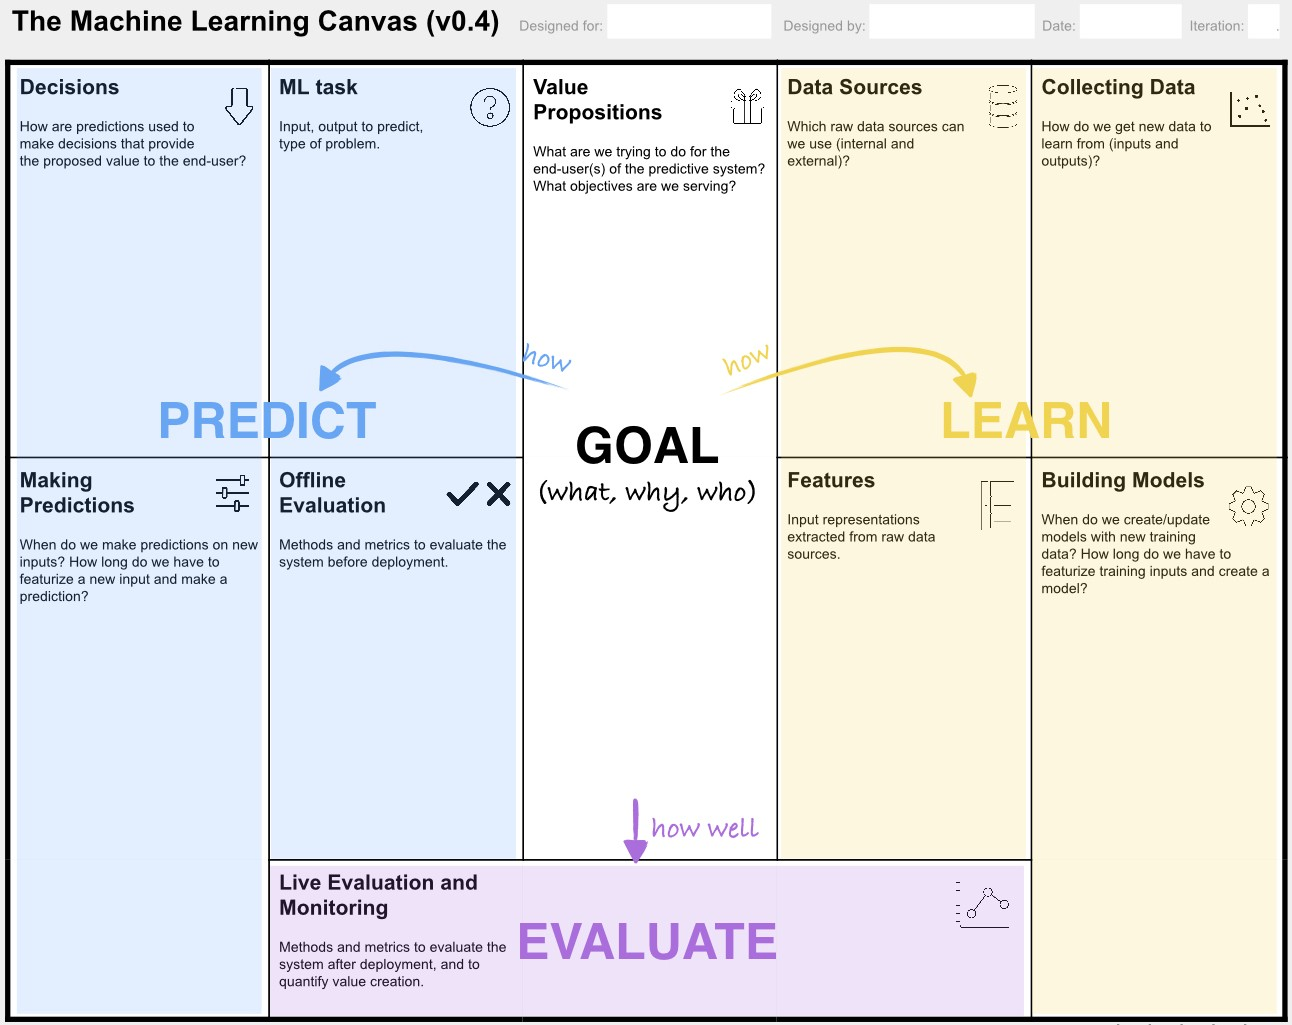
\includegraphics[width=0.8\textwidth]{images/ml_canvas.jpeg}
  \caption{``The Machine Learning Canvas'' \cite{dorad_machine_2016}.}
  \label{fig:ml_canvas}
\end{figure}

\paragraph{}
Il est important de noter que cette feuille ne peut pas être complété par un développeur seul ou par le commanditaire, les deux profils sont essentiels. De plus, cet outil à pour avantage d'être lisible par un nouvel acteur qui pourrait rentrer dans le projet.

\subsection{Analyse de l'impact environnemental d'un modèle}

\paragraph{}
Dans cette partie nous allons voir deux outils : une librairie du langage Python qui mesure l'impact du calcul de l'exécution d'une fonction (energy-usage\footnote{https://github.com/responsibleproblemsolving/energy-usage}) et une interface web pouvant qui calcule les émissions en CO2 en fonction du temps d'entraînement et du matériel utilisé (ML CO2 Impact\footnote{https://mlco2.github.io/impact/}).

\subsubsection{energy-usage}

\paragraph{}
Cette librairie Python permet d'avoir un certain nombre d'informations concernant l'impact environnemental du calcul de fonction écrit dans ce même langage informatique de Python. Dans la pratique il suffit de construire une fonction et de l'appliquer avec l'outil, un rapport sera généré avec les informations suivantes : la puissance moyenne utilisée (en Watt) avec et sans le processus, la durée d'exécution, les sources d'énergies selon la géolocalisation, les émissions CO2, des comparaisons et enfin la quantité d'énergies utilisées par le programme (en kWh).

\paragraph{}
Afin de calculer avec précision les émissions de CO2 associées à la puissance de calcul utilisée, ils déterminent la localisation géographique de l'utilisateur via son adresse IP à l'aide de l'API GeoJS\footnote{https://www.geojs.io/}. Si la localisation ne peut pas être déterminée, les USA sont utilisés par défaut.

\paragraph{}
La localisation est particulièrement importante car les émissions diffèrent en fonction de la combinaison énergétique du pays (et, dans le cas des États-Unis, de l'État). Ils ont obtenus les mixes des sources d'énergies en examinant la consommation d'énergie des pays du monde entier, ventilée par source d'énergie.

\paragraph{}
Au cas où nous souhaitont comparer la consommation d'énergie entre différentes années de données, ils ont inclus un script pour permettre d'ajouter d'autres années.

\paragraph{}
Cet outil est donc assez complet, mais a pour défaut de ne pas pouvoir être exécuté sur n'importe quel environnement de travail. Il sera donc pertinent de réaliser différentes exécutions sur environnement valide pour permettre à un utilisateur ne pouvant pas l'utiliser d'estimer la consommation de sa fonction dans son environnement.

\subsubsection{ML CO2 Impact}

\begin{quotation}
  ``Une grande puissance de calcul s'accompagne d'une grande responsabilité''
\end{quotation}
\rightline{{\rm --- \citep{lacoste2019quantifying}}} 

\paragraph{}
``Machine Learning CO2 Impact'' est un outil disponible par un site internet, contrairement à l'outil précédent il se centralise sur la consommation énergétique de l'entraînement d'un modèle de Machine Learning. De pkus, cet outil a pour atout de prendre en compte des fournisseurs de Cloud en fonction de leur région, ce qui au vu de l'évolution de l'utilisation des technologies sur ces plateformes est un grand atout.

\paragraph{}
L'ajout intéressant du site est la section ``There are things you can do''\footnote{Traduction : Il y a des choses que vous pouvez faire.}. En effet, ils recommandent les suggestions suivantes : 
\begin{itemize}
  \item Choisir judicieusement son fournisseur Cloud : Ils n'achètent pas tous des compensations, des REC\footnote{REC : Renewable Energy Credits signifiant Crédits d'énergies renouvelables} ou n'investissent pas tous de la même façon dans les sources d'énergie propres. Lire leurs engagements en matière de durabilité et faites un choix éclairé.
  \item Choisir sa région : Les différentes régions sont alimentées par différentes combinaisons d'énergies renouvelables et non renouvelables. Si la réglementation et les aspects juridiques le permettent, choisissez une région plus durable.
  \item Acheter des compensations carbone : De nombreuses plateformes proposent des moyens simples de compenser les émissions. Il est possible d'avoir un impact important en proposant des compensations au sein de votre organisation. 
  \item Ne pas utiliser de recherche par grille\footnote{Cette méthode consiste à choisir un algorithme et d'essayer une grande quantité de combinaison d'hyperparamètres (paramètres de l'algorithme) jusqu'à trouver la meilleure combinaison d'entrâinement.} : La recherche par hyperparamètres est une grande source d'émissions de carbone liées au Machine Learning. S'il n'existe pas de documentation pour aider à établir de bonnes valeurs et que la recherche des valeurs pertinentes est nécessaire, le faire au moins de manière aléatoire, et non par le biais d'une recherche par grille.
  \item Choisir l'énergie propre : Une organisation peut avoir le choix de son alimentation électrique. Le choix d'une source d'énergie plus propre et plus durable contribuera grandement à réduire votre impact carbone
\end{itemize}

\paragraph{}
L'inconvénient de cet outil est qu'il est utilisable que sur l'adresse web indiquée et par conséquent il est très difficile de l'implémenter dans un outil externe.

\section{TransparentAI : de la théorie à la pratique}

\paragraph{}
Pour rappel, avec le grand nombre de publications pour définir ce que devrait être une intelligence artificielle éthique, mais sans aborder l'aspect technique de cette question il y a une frustration des développeurs de ces algorithmes. Nous avons donc bien identifié le problème : comment passer de la théorie à la pratique ou pour citer la problématique de ce mémoire est-il possible de rendre une Intelligence Artificielle socialement responsable en supervisant son éthique ?

\paragraph{}
Dans ce contexte, nous avons également identifié que sur le plan technique, il existe bel et bien des outils qui réponde à des aspects évoqués dans les documents comme l'évaluation des biais injustes, l'impact environnemental d'un modèle ou encore l'explication du comportement d'un modèle.

\paragraph{}
C'est ici que rentre en jeu l'outil nommé TransparentAI, qui comme son nom l'indique vise à tendre vers une intelligence artificielle transparente ou selon la Commission Européenne, de confiance. J'ai fait le choix de créer cet outil dans le but d'allier la théorie d'une IA de confiance selon la Commssion Européenne directement avec les réponses techniques déjà disponibles et libre d'accès. 

\subsection{Finalité : évaluer l'éthique d'une IA}

\paragraph{}
Reprenons ce qui définit la théorie derrière une intelligence artificielle de confiance : les sept exigences de la Commission Européenne. Chacune de ces exigences à plusieurs aspects expliquant à quoi elle correspond. La première étape pour superviser l'éthique d'une IA est donc de dérouler chacun des aspects et de définir comment répondre au fondamental éthique sous-jacent. Par exemple, pour l'exigence de l'Action humaine et du contrôle humain, l'un des aspect correspond au respect des droits fondamentaux, or, cela n'est pas vérifiable techniquement, c'est un mélange de connaissance juridique et métier. La réponse à apporter dans ce contexte est déclarative et se doit de répondre à des questions commes  ``Dans les cas d’utilisation susceptibles d’entraîner des effets négatifs sur les droits fondamentaux, avez-vous réalisé une analyse d’impact sur les droits fondamentaux ?'' \citep{commission_europeenne_ethics_2019}.

\paragraph{}
Nous avons donc besoin d'une liste des aspects avec des questions pouvant permettre de contrôler facilement si l'aspect respecte la notion d'IA de confiance. Pour une partie des aspects dérivés des exigences, la difficulté vient du fait de ne pas être vérifié par le biais d'une réponse déclarative. Parfois, il est nécessaire d'aller contrôler avec des méthodes techique comme celles présentées dans la section précédente. Partant de cela, nous pouvons, pour chaque exigence, définir à partir des aspects listés par la Commission Européenne, dresser les questions pouvant s'assurer de la confiance d'une IA. De plus, nous pouvons également ajouter si une implémentation technique est possible pour chaque aspect.

\paragraph{1. Action humaine et contrôle humain}

\begin{center}
  \begin{tabular}{ |p{4cm}|p{6cm}|p{2cm}| } 
    \hline
    Aspect & Question & Tech ? \\
    \hline
    \hline
    Droits fondamentaux &  & Non \\
    \hline
    Action humaine & & Non \\
    \hline
    Contrôle humain & & Non \\ 
    \hline
    
  \end{tabular}
\end{center}

\paragraph{2. Robustesse technique et sécurité}

\begin{center}
  \begin{tabular}{ |p{4cm}|p{6cm}|p{2cm}| } 
    \hline
    Aspect & Question & Tech ? \\
    \hline
    \hline
    Résilience aux attaques et sécurité &  & Non \\
    \hline
    Solutions de secours et sécurité générale &  & Non \\
    \hline
    Précision &  & Non \\
    \hline
    Fiabilité et reproductibilité &  & Non \\
    \hline
    
  \end{tabular}
\end{center}

\paragraph{3. Respect de la vie privée et gouvernance des données}

\begin{center}
  \begin{tabular}{ |p{4cm}|p{6cm}|p{2cm}| } 
    \hline
    Aspect & Question & Tech ? \\
    \hline
    \hline
    Respect de la vie privée et protection des données &  & Non \\
    \hline
    Qualité et intégrité des données &  & Non \\
    \hline
    Accès aux données &  & Non \\
    \hline
    
  \end{tabular}
\end{center}

\paragraph{4. Transparence}

\begin{center}
  \begin{tabular}{ |p{4cm}|p{6cm}|p{2cm}| } 
    \hline
    Aspect & Question & Tech ? \\
    \hline
    \hline
    Traçabilité &  & Non \\
    \hline
    Explicabilité &  & Non \\
    \hline
    Communication &  & Non \\
    \hline
    
  \end{tabular}
\end{center}

\paragraph{5. Diversité, non-discrimination et équité}

\begin{center}
  \begin{tabular}{ |p{4cm}|p{6cm}|p{2cm}| } 
    \hline
    Aspect & Question & Tech ? \\
    \hline
    \hline
    Éviter les biais injustes &  & Non \\
    \hline
    Accessibilité et conception universelle &  & Non \\
    \hline
    Participation des parties prenantes &  & Non \\
    \hline
    
  \end{tabular}
\end{center}

\paragraph{6. Bien-être sociétal et environnemental}

\begin{center}
  \begin{tabular}{ |p{4cm}|p{6cm}|p{2cm}| } 
    \hline
    Aspect & Question & Tech ? \\
    \hline
    \hline
    IA durable et respectueuse de l’environnement &  & Non \\
    \hline
    Incidence sociale &  & Non \\
    \hline
    Société et démocratie &  & Non \\
    \hline
    
  \end{tabular}
\end{center}

\paragraph{7. Responsabilité}

\begin{center}
  \begin{tabular}{ |p{4cm}|p{6cm}|p{2cm}| } 
    \hline
    Aspect & Question & Tech ? \\
    \hline
    \hline
    Auditabilité &  & Non \\
    \hline
    Minimisation et documentation des incidences négatives &  & Non \\
    \hline
    Documentation des arbitrages &  & Non \\
    \hline
    Voies de recours &  & Non \\
    \hline
    
  \end{tabular}
\end{center}

\paragraph{}
Au vu de ces questions, nous contastons que majoritairement deux profils sont requis afin de bien compléter ce formulaire de question : un profil métier (le commanditaire du projet ou le chef de projet par exemple) et un profil technique comme un data scientist. Nous allons donc voir dans la section suivante comment se construit l'outil de TransparentAI et pourquoi.

\subsection{Structure technique}

\subsubsection{Un outil orienté technique : une librairie Python}

Découpage en sous modules qui peuvent être lié aux exigences

\subsubsection{Un outil orienté métier : une interface web}


\section{Synthèse}


% ======= PLAN DE RECHERCHE ===== %
\newpage
\chapter{Plan de recherche}


\paragraph{Problématique :}
Est-il possible de rendre une Intelligence Artificielle socialement responsable en supervisant son éthique ?

\paragraph{Hypothèse}
MH = Morale humaine définie sur les attributs sociaux 
MAI = Morale IA inconnue (à analyser)
S = Scénario pouvant être présenté à l'entrée d'une IA
A = Action issu d'un scénario S et amenant un résultat R
R = Résultat d'une IA utilisant des données en entrée spécifique.

- H1 : A partir d'une morale MH et une intelligence artificielle ayant une morale MAI, il est possible d'identifier si MH est aligné avec MAI afin de respecter l'équation MH ~= MAI.
- H2 : L'utilisation de TransparentAI permet de garantir un alignement avec les valeurs théoriques d'une IA de confiance définie par la Commission Européenne.
- H3 : Avec un scénario S défini, il est possible de comprendre l'action A amenant au résultat R.
- H4 : Si MH != MAI alors il est possible d'atténuer voire annuler les biais afin de respecter l'équation MH ~= MAI.

\paragraph{Expérience}

Objectif
Un objectif sensible bancaire : 
prédire la probabilité qu'un client puisse rembourser un prêt ?

Données
Utilisation des données de la compétition Kaggle : https://www.kaggle.com/c/home-credit-default-risk/overview/description

Mesure du succès 
Choix de la mesure :  M
Seuil minimum : T

Justification :

\paragraph{Définition des morales}
M = mesure de performance du modèle 
T = Seuil minimum
P = Probabilité de rembourser un prêt
PF = Probabilité qu'une femme puisse rembourser un prêt
X = variable selon morale

- Alice : pour l'équation M >= T + X, maximiser X
- Bob : en respectant M >= T, discriminer le groupe social GENRE en défavorisant les femmes en suivant l'équation suivante : PF = P - X, en maximisant X
- Charlie : en respectant M >= T, discriminer le groupe social GENRE en favorisant les femmes en suivant l'équation suivante : PF = P + X, en maximisant X
- Morale de Contrôle : en respectant M >= T, créer un algorithme simple sans prendre en compte les attributs sociaux

\paragraph{Processus}
Création des IA : création d'un repo GitHub avec env Docker
- Pour Alice : utiliser code Kaggle déjà performant

Validation par le même processus : mesure M respectant M >= S

Analyse des biais en utilisant TransparentAI : constatation des résultats pour les 4 morales

Proposition de réduction de biais ou amplification à partir de chaque Morale vers une autre

Application des algorithmes de réduction

Nouvelle analyse de performance + biais

\paragraph{Limites} 
- reste déclaratif rien n'est imposé
- possible d'identifier les biais, de les atténuer ou pas
- 

\section{Définition des hypothèses}

\section{Environnement de recherche}

\subsection{Contexte : prédire la probabilité de rembourser un prêt}

\subsection{Algorithmes choisis}

% ======= EXPERIENCE ===== %
\newpage
\chapter{Expérience}

\section{Réalisation de l'expérience}

\section{Résultats obtenus}

\section{Conclusion de l'expérience}

% ====== CONCLUSION ====== %

\newpage
\chapter*{Conclusion}
\addcontentsline{toc}{chapter}{\protect\numberline{}Conclusion}

\newpage
% \bibliographystyle{alpha}
\bibliographystyle{plainnat}
\bibliography{bibliography}

\end{document}